\Appendix{Derivation of Transverse Emittance} \label{apx:emittance}

The following is a derivation of Eq. \eqref{eqn:emittancedef}. First, it is assumed that the beam is an on-axis Gaussian beam. Explicitly, this is to say that the distribution of transverse coordinates is Gaussian and that $\left(\left<x\right>,\left<\theta\right>\right)=(0,0)$. Recall that emittance is a measure of phase space volume. To measure this volume, it is necessary to use a bivariate Gaussian distribution.

In general, a multivariate Gaussian distribution has the form
\begin{equation}\nonumber
f_n (X)=\frac{1}{(2\pi)^{n/2}|\mathcal{A}|^{1/2}}\exp\left(-\frac{1}{2}(X-\mu)^T\mathcal{A}^{-1}(X-\mu)\right),
\end{equation}
where $X=(x_1,...,x_n)$ is a column vector of independent variables, $\mathcal{A}\in S^n_{++}$ is the covariance matrix, and $\mu=(\mu_1,...,\mu_n)$ is a column vector of average values (which are all zero for this derivation) \cite{Do}. $S^n_{++}$ is the space of symmetric positive definite $n\times n$ matrices.  The covariance matrix $\mathcal{A}$ is a matrix that describes the covariance between variables. That is, $\mathcal{A}$ describes how much two given variables change with one another.

As an example, consider the univariate Gaussian distribution. The only variable is $x$ and it changes with itself as $\left<x\cdot x\right> = \sigma^2$. Then
\begin{align*}
X=x,\qquad\mathcal{A}=\sigma^2,
\end{align*}
and
\begin{align*}
f_1 (X)&=\frac{1}{(2\pi)^{1/2}\sigma} \exp\left(-\frac{1}{2}x\frac{1}{\sigma^2}x\right)\\
&=\frac{1}{\sqrt{2\pi}\sigma} \exp\left(-\frac{x^2}{2\sigma^2}\right).
\end{align*}

For the transverse emittance, there are two varibles, $x$ and $\theta$. They change with themselves as their respective $\sigma^2$ and with one another as $\left<x\theta\right>$, and so
\begin{align*}
X=(x,\theta)\qquad\mathcal{A}=\begin{pmatrix}
					\sigma_x^2 & \left<x\theta\right>\\
					\left<x\theta\right> & \sigma_\theta^2
					\end{pmatrix}.
\end{align*}

The distribution is
\begin{align*}
f_2(X)&=\frac{1}{2\pi\sqrt{\sigma_x^2\sigma_\theta^2-\left<x\theta\right>^2}}\exp\left(-\frac{x^2\sigma_\theta^2-2x\theta\left<x\theta\right>+\theta^2\sigma_x^2}{2(\sigma_x^2\sigma_\theta^2-\left<x\theta\right>^2)}\right).
\end{align*}
Since the boundary of this function is undefined, it is conventional to use a metric called the Mahalanobis distance \cite{mahalanobis}. This is a measure of how far some point is away from the center of a multivariate distribution. For a bivariate Gaussian distribution, it is
\begin{align*}
\text{distance}=\frac{1}{2}(X-\mu)^T\mathcal{A}^{-1}(X-\mu)=\frac{x^2\sigma_\theta^2-2x\theta\left<x\theta\right>+\theta^2\sigma_x^2}{2(\sigma_x^2\sigma_\theta^2-\left<x\theta\right>^2)}.
\end{align*} 
As it pertains to emittance, the boundary of interest is all $x$ and $\theta$ combinations which are unit distance from the central peak. Then
\begin{align*}
1=\frac{x^2\sigma_\theta^2-2x\theta\left<x\theta\right>+\theta^2\sigma_x^2}{2(\sigma_x^2\sigma_\theta^2-\left<x\theta\right>^2)}.
\end{align*}

Now it is apparent that this equation represents an ellipse in $x-\theta$ phase space:
\begin{align} \label{eqn:ellipse}
1=Ax^2+2Bx\theta+C\theta^2,
\end{align}
with
\begin{align*}
A&=\sigma_\theta^2/D,\\
B&=-\left<x\theta\right>/D,\\
C&=\sigma_x^2/D,\\
D&=2(\sigma_x ^2 \sigma_\theta^2 - \left<x\theta\right>^2).
\end{align*}

Indeed, an ellipse is exactly what one would expect. Observe from Figure~\ref{fig:bivariate_ellipse} that the projection of equal heights from a bivariate Gaussian onto the $x-\theta$ plane is an ellipse. This ellipse can get bigger or smaller depending on the Mahalanobis distance chosen, with the extrema being 0 and $\infty$.

\begin{figure}
  \centering
    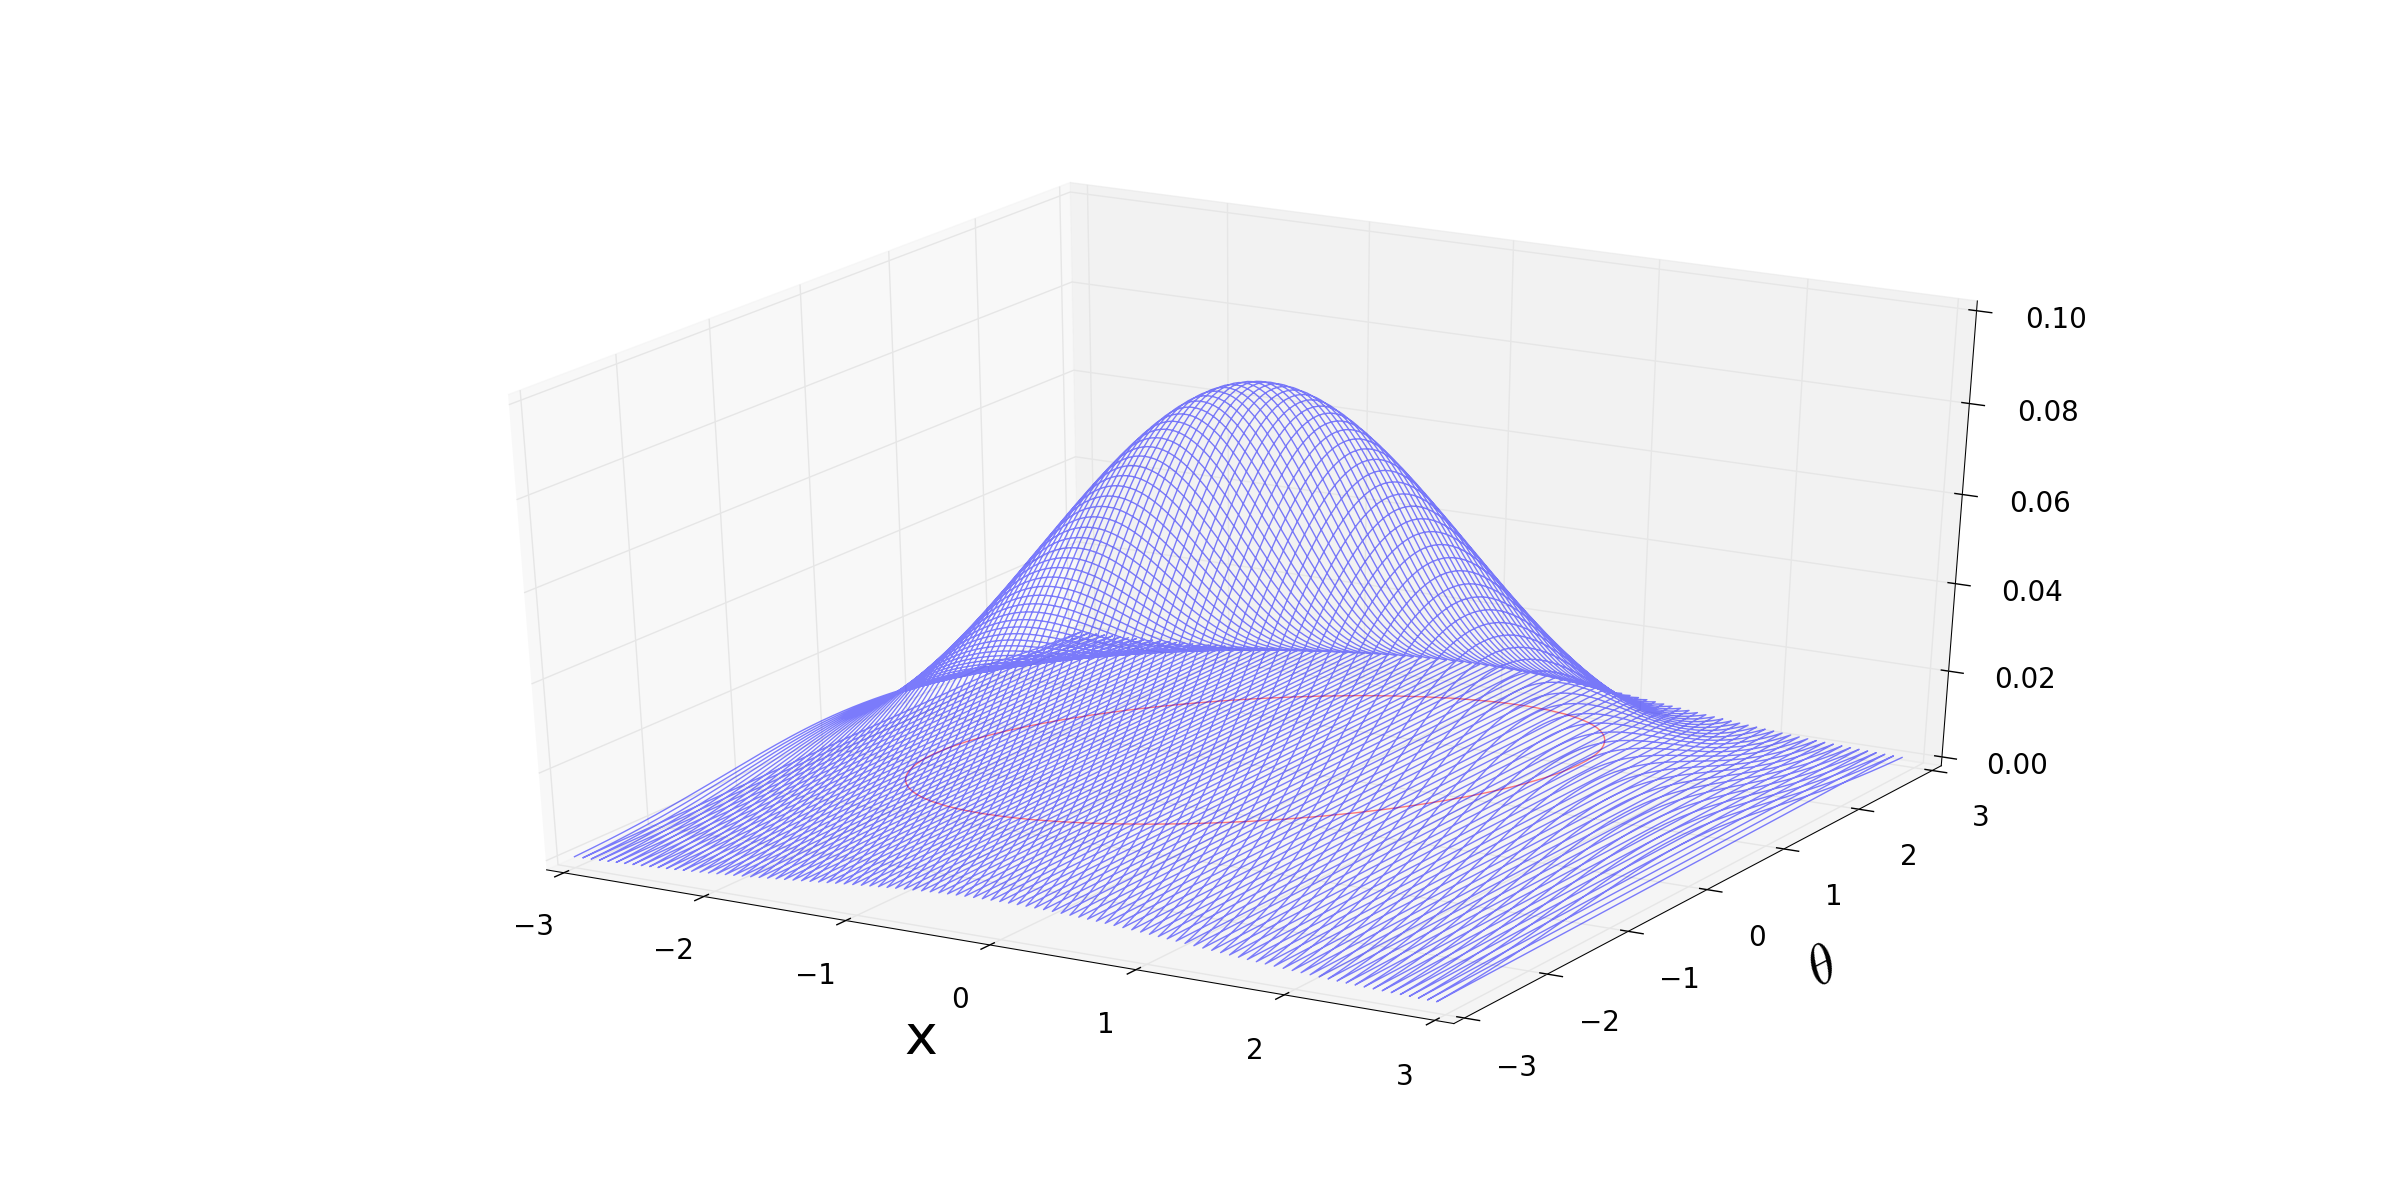
\includegraphics[width=\textwidth]{Figures/bivariate_ellipse} 
  \caption[Sample scatterplot of a bivariate Gaussian with its projected ellipse.]{Sample scatterplot of a bivariate Gaussian (blue). The ellipse (red) is a projection of points of equal heights onto the $x-\theta$ plane.}
  \label{fig:bivariate_ellipse}
\end{figure}

The area of this ellipse is the emittance (the volume of phase space) that is desired. For an untilted ellipse, this area is equal to $\pi$ times the length of the major axis ($a$) times the length of the minor axis ($b$), or $\text{Area}=\pi a b$. The goal, then, is to apply a transformation of coordinates to the (potentially) tilted ellipse. This transformation to a new coordinate system ($x'$, $\theta '$) is a simple rotation such that the major and minor axes of the ellipse are coincident with the $x'$ and $\theta '$ axes. Then it is much easier to find the major and minor axis lengths.

Note that Eq. \eqref{eqn:ellipse} can also be represented by
\begin{align*}
1=\begin{pmatrix} x & \theta \end{pmatrix}	\mathcal{B} 	\begin{pmatrix} x\\ \theta \end{pmatrix}
\end{align*}
where
\begin{align*}
\mathcal{B}=
	\begin{pmatrix}
	A & B\\
	B & C
	\end{pmatrix}.
\end{align*}
This is a useful representation, since the ``normal'' form (with the ellipse aligned to the $x'$ and $\theta '$ axes) is desired:
\begin{align} \label{eqn:ellipse_normal_form}
1 = A'x'^2 + C'\theta '^2,
\end{align}
or equivalently
\begin{align*}
1 = \begin{pmatrix} x' & \theta ' \end{pmatrix}	\mathcal{B'} 	\begin{pmatrix} x'\\ \theta ' \end{pmatrix}
\end{align*}
with
\begin{align*}
\mathcal{B}'=\begin{pmatrix} A' & 0 \\ 0 & C' \end{pmatrix}.
\end{align*}
The goal, then, is to diagonalize $\mathcal{B}$. The diagonalization may be done via finding the eigenvalues and eigenvectors or by introducing some angle that relates $x'$ and $\theta '$ to $x$ and $\theta$. Regardless, the result is
\begin{align*}
A'&=\frac{1}{2}\left(A+C+\sqrt{A^2-2AC+C^2+4B^2}\right)\\
C'&=\frac{1}{2}\left(A+C-\sqrt{A^2-2AC+C^2+4B^2}\right).
\end{align*}

In accordance with Eq. \eqref{eqn:ellipse_normal_form}, the major and minor axis lengths are given by $1/2\sqrt{A'}$ and $1/2\sqrt{C'}$\footnote{It may help to recall that the normal form equation for an ellipse may also be represented by $\frac{x^2}{a^2}+\frac{y^2}{b^2}=1$, where $a$ and $b$ are the major or minor axis half-lengths.}. Then the area of the ellipse in question is
\begin{align*}
\text{Area}&=\pi\frac{1}{2\sqrt{A'}}\frac{1}{2\sqrt{C'}}
&=\pi\sqrt{\sigma_x^2\sigma_\theta^2 - \left<x\theta\right>^2}.
\end{align*}
For the emittance, the $\pi$ term is usually absorbed into the units (e.g. millimeter pi radians), and so the emittance is simply
\begin{equation}\label{emittance_appendix}
\epsilon=\sqrt{\sigma_x^2\sigma_\theta^2 - \left<x\theta\right>^2}.
\end{equation}


 %----------------------------------------------------------------------------------------------------------------------
\Appendix{Derivation of Implemented Scattering Cross Section}\label{apx:cosy_cross_section}
 Electron-muon scattering is a textbook scattering problem following Feynman rules \cite{griffithspp}. Similar to both Section~\ref{sec:ICOOLStraggling} and Section~\ref{sec:ICOOLScattering}, either the collision time of the muon and electron is assumed to be very small compared to the electron orbital time or the electron is initially at rest. The longitudinal ($z$) axis is aligned with the muon velocity such that $v_x=v_y=0$. The reference frame is the lab frame. Please refer to the information in Appendix~\ref{apx:particlePhysicsReview} for a review on symbols and methods.

To find the (differential) scattering cross section $d\sigma/d\Omega$, it is necessary to have both the scattering amplitude $\mathcal{M}$ (sometimes also called the `matrix element', although this is a little ambiguous) and the available phase space over which to integrate. However, \cite{griffithspp} notes that the integration over the available phase space is a constant, and so only the scattering amplitude is of interest.

Recall that the desired cross section is the Rutherford-like tail of a Gaussian--Rutherford-like piecewise function. The multiplicative constants are ignored since only the forms of the individual Gaussian and Rutherford-like functions are desired. Then
\begin{align*}
\frac{d\sigma}{d\Omega}\propto |\mathcal{M}|^2.
\end{align*}

To find the scattering amplitude $\mathcal{M}$, observe that Figure~\ref{fig:mottFeynman} represents a muon-electron interaction via exchange of a virtual photon from the electron vertex $\alpha$ to the muon vertex $\beta$. The fermion flow is the path which goes along the directions of the arrows. For example, the first fermion flow which is observed is the muon flow: a muon enters from the left, there is an interaction at the propagator vertex $\beta$, and a muon exits from the right. Each muon contributes its spinor. The outgoing muon and incoming muon are adjoints of one another (i.e. if the spinor of $P_2$ is $U(P_2)$ then the spinor of $P_4$ is $\bar{U}(P_4)$). The propagator vertex contributes a factor of $-ieQ_\mu\gamma^\beta$. Since matrices compound right-to-left, it is necessary to start at the end of the fermion flow and work backwards. Figure~\ref{fig:mottFeynmanMath} helps to show that the scattering amplitude is
\begin{equation} \label{eqn:mottFeynmanScatteringAmplitude}
i\mathcal{M}=\bar{U}_4(-ieQ_\mu\gamma^\beta)U_2\cdot\frac{i}{q^2}(-\eta_{\alpha\beta}+\frac{q_\alpha q_\beta}{q^2})\cdot\bar{U}_3(-ieQ_e\gamma^\alpha)U_1,
\end{equation}
where $U_i$ is the spinor for the $i^{th}$ particle, $q$ is the momentum carried by the virtual photon, $\gamma^i$ is the $\gamma$ matrix corresponding to vertix $i$ in Figure~\ref{fig:mottFeynman}, $\alpha,\beta$ denote the vertices in Figure~\ref{fig:mottFeynman}, and $\eta_{i,j}$ is the $(i,j)^{th}$ component of the Minkowski metric described in Section~\ref{ssc:griffithsRule12}.

\begin{figure}
  \centering
    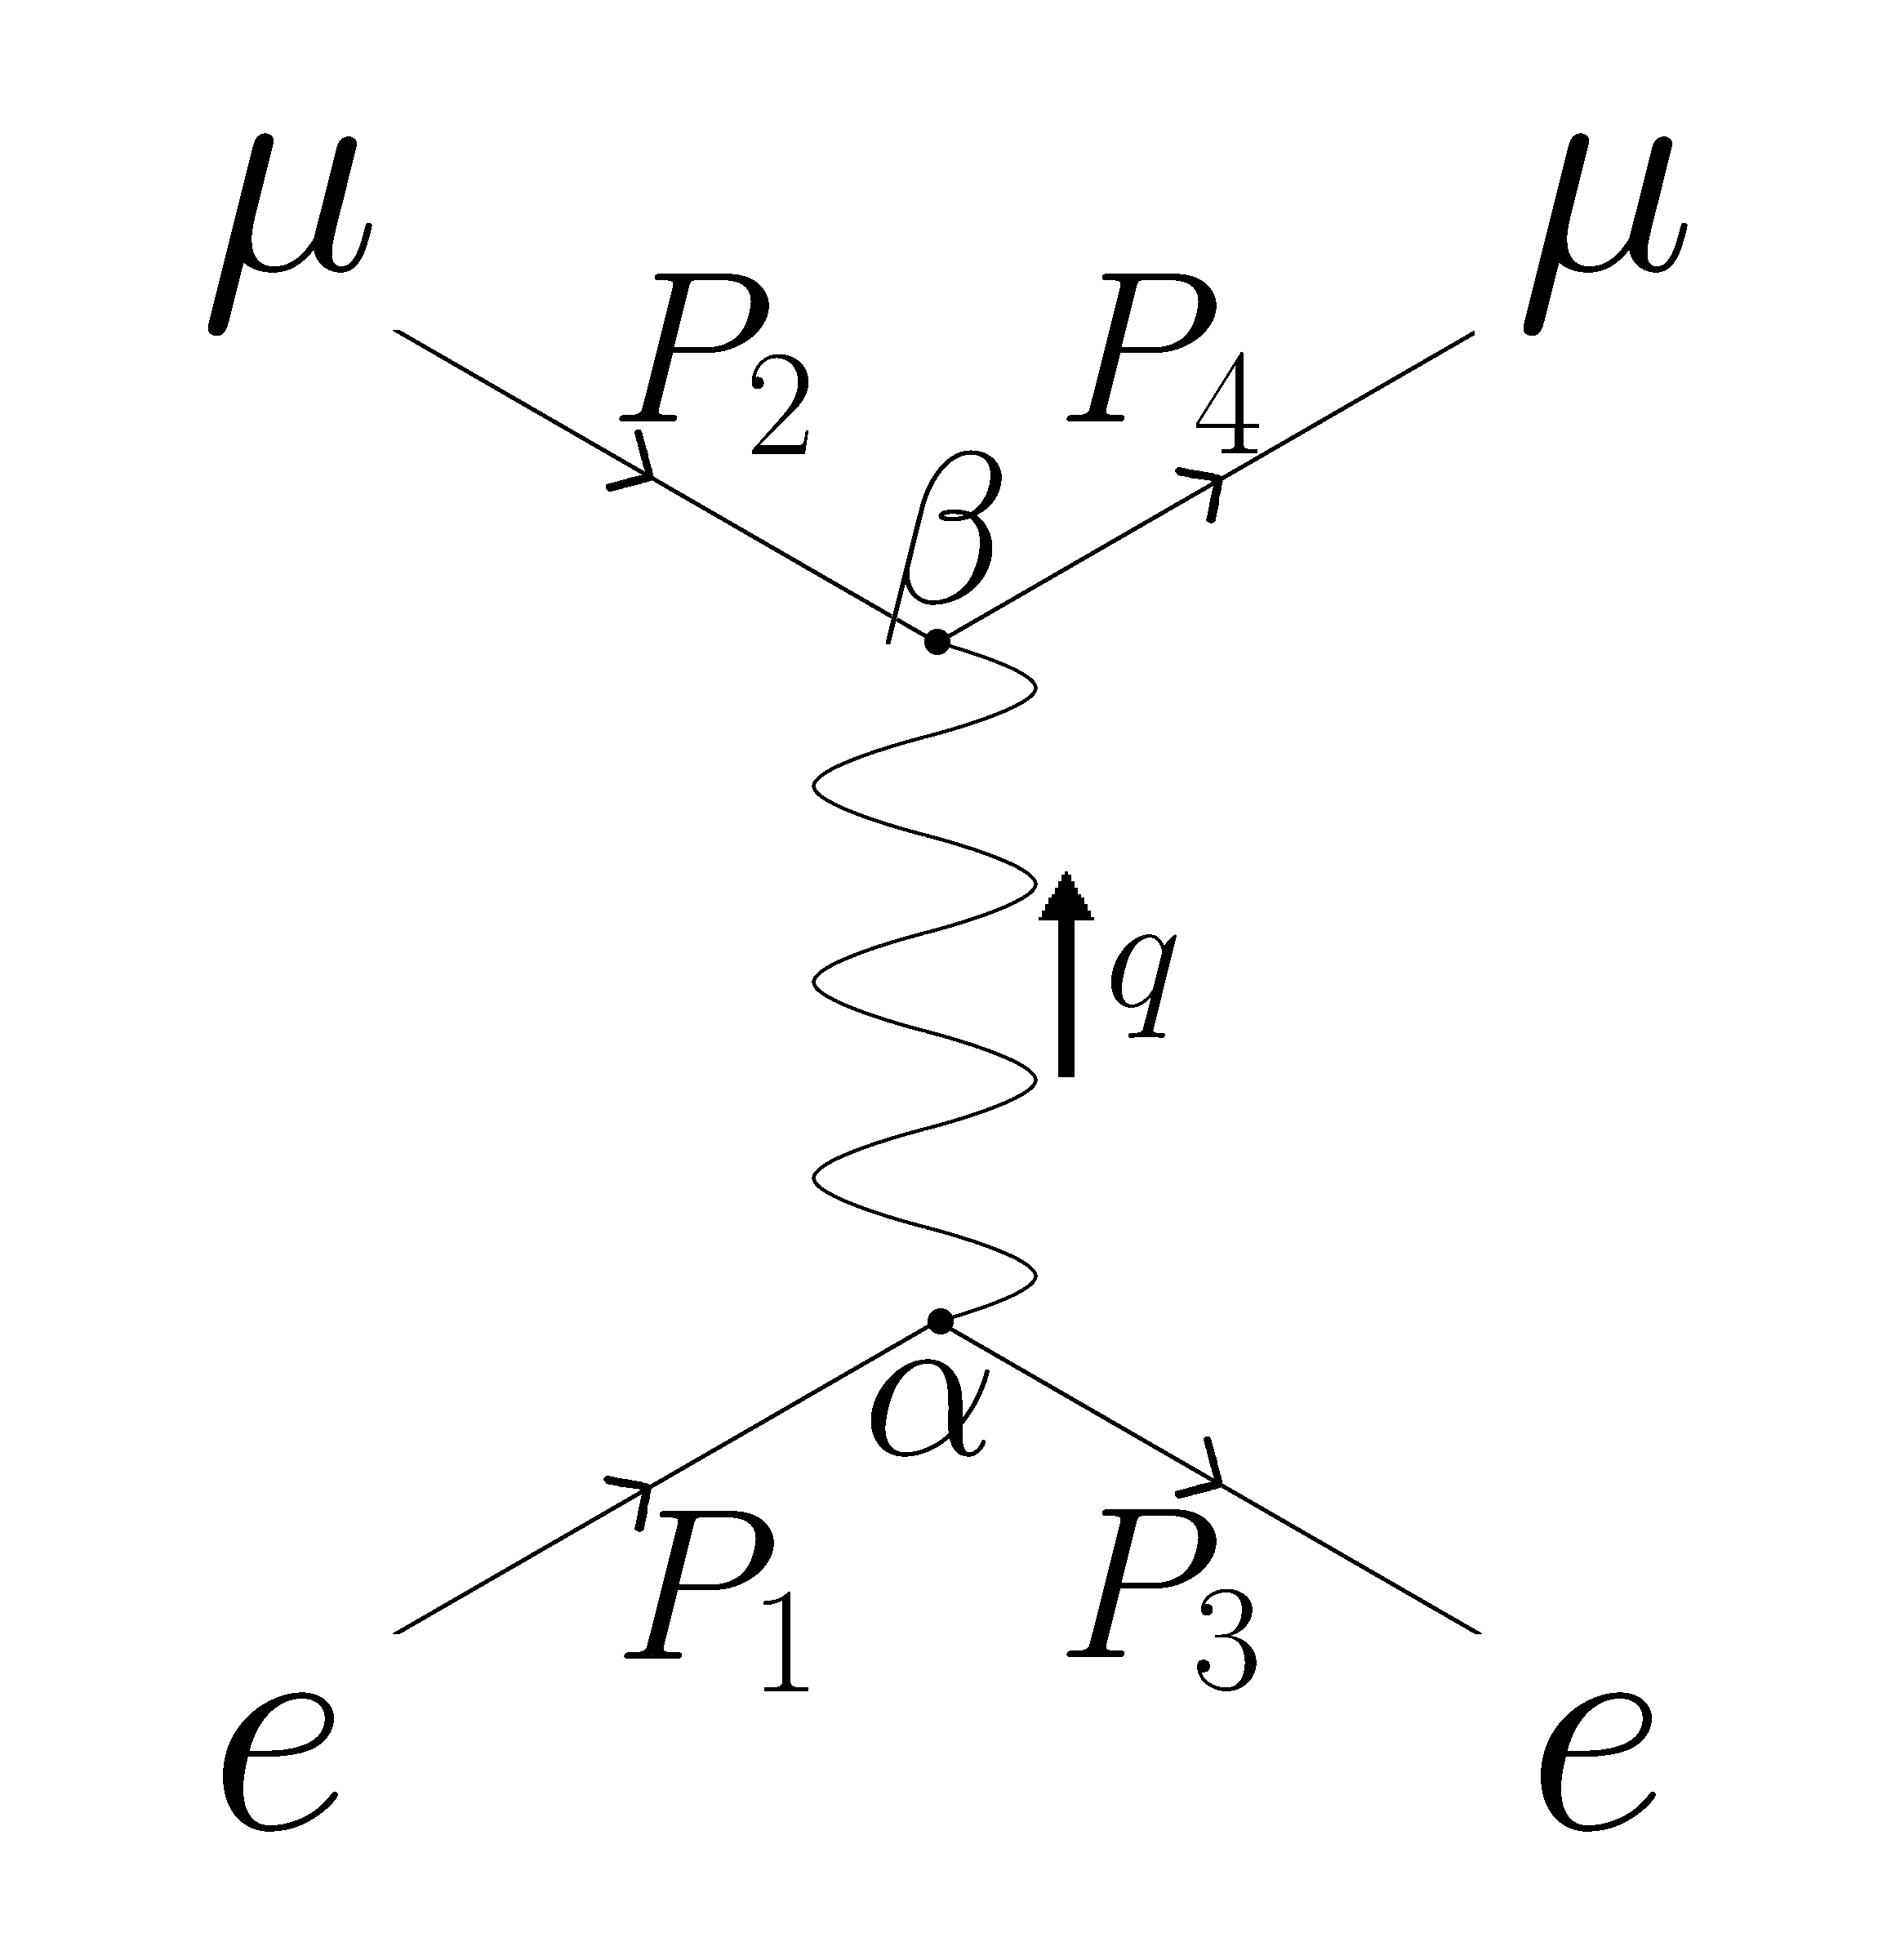
\includegraphics[width=0.5\textwidth]{Figures/MottFeynman} 
  \caption[Feynman diagram for electron-muon scattering.]{Feynman diagram for electron-muon scattering. $P_1$ and $P_2$ are the incoming four-momenta for the electron and muon and $P_3$ and $P_4$ are the outgoing four-momenta. $q$ represents the four-momentum carried by the virtual photon.}
  \label{fig:mottFeynman}
\end{figure}

\begin{figure}
  \centering
    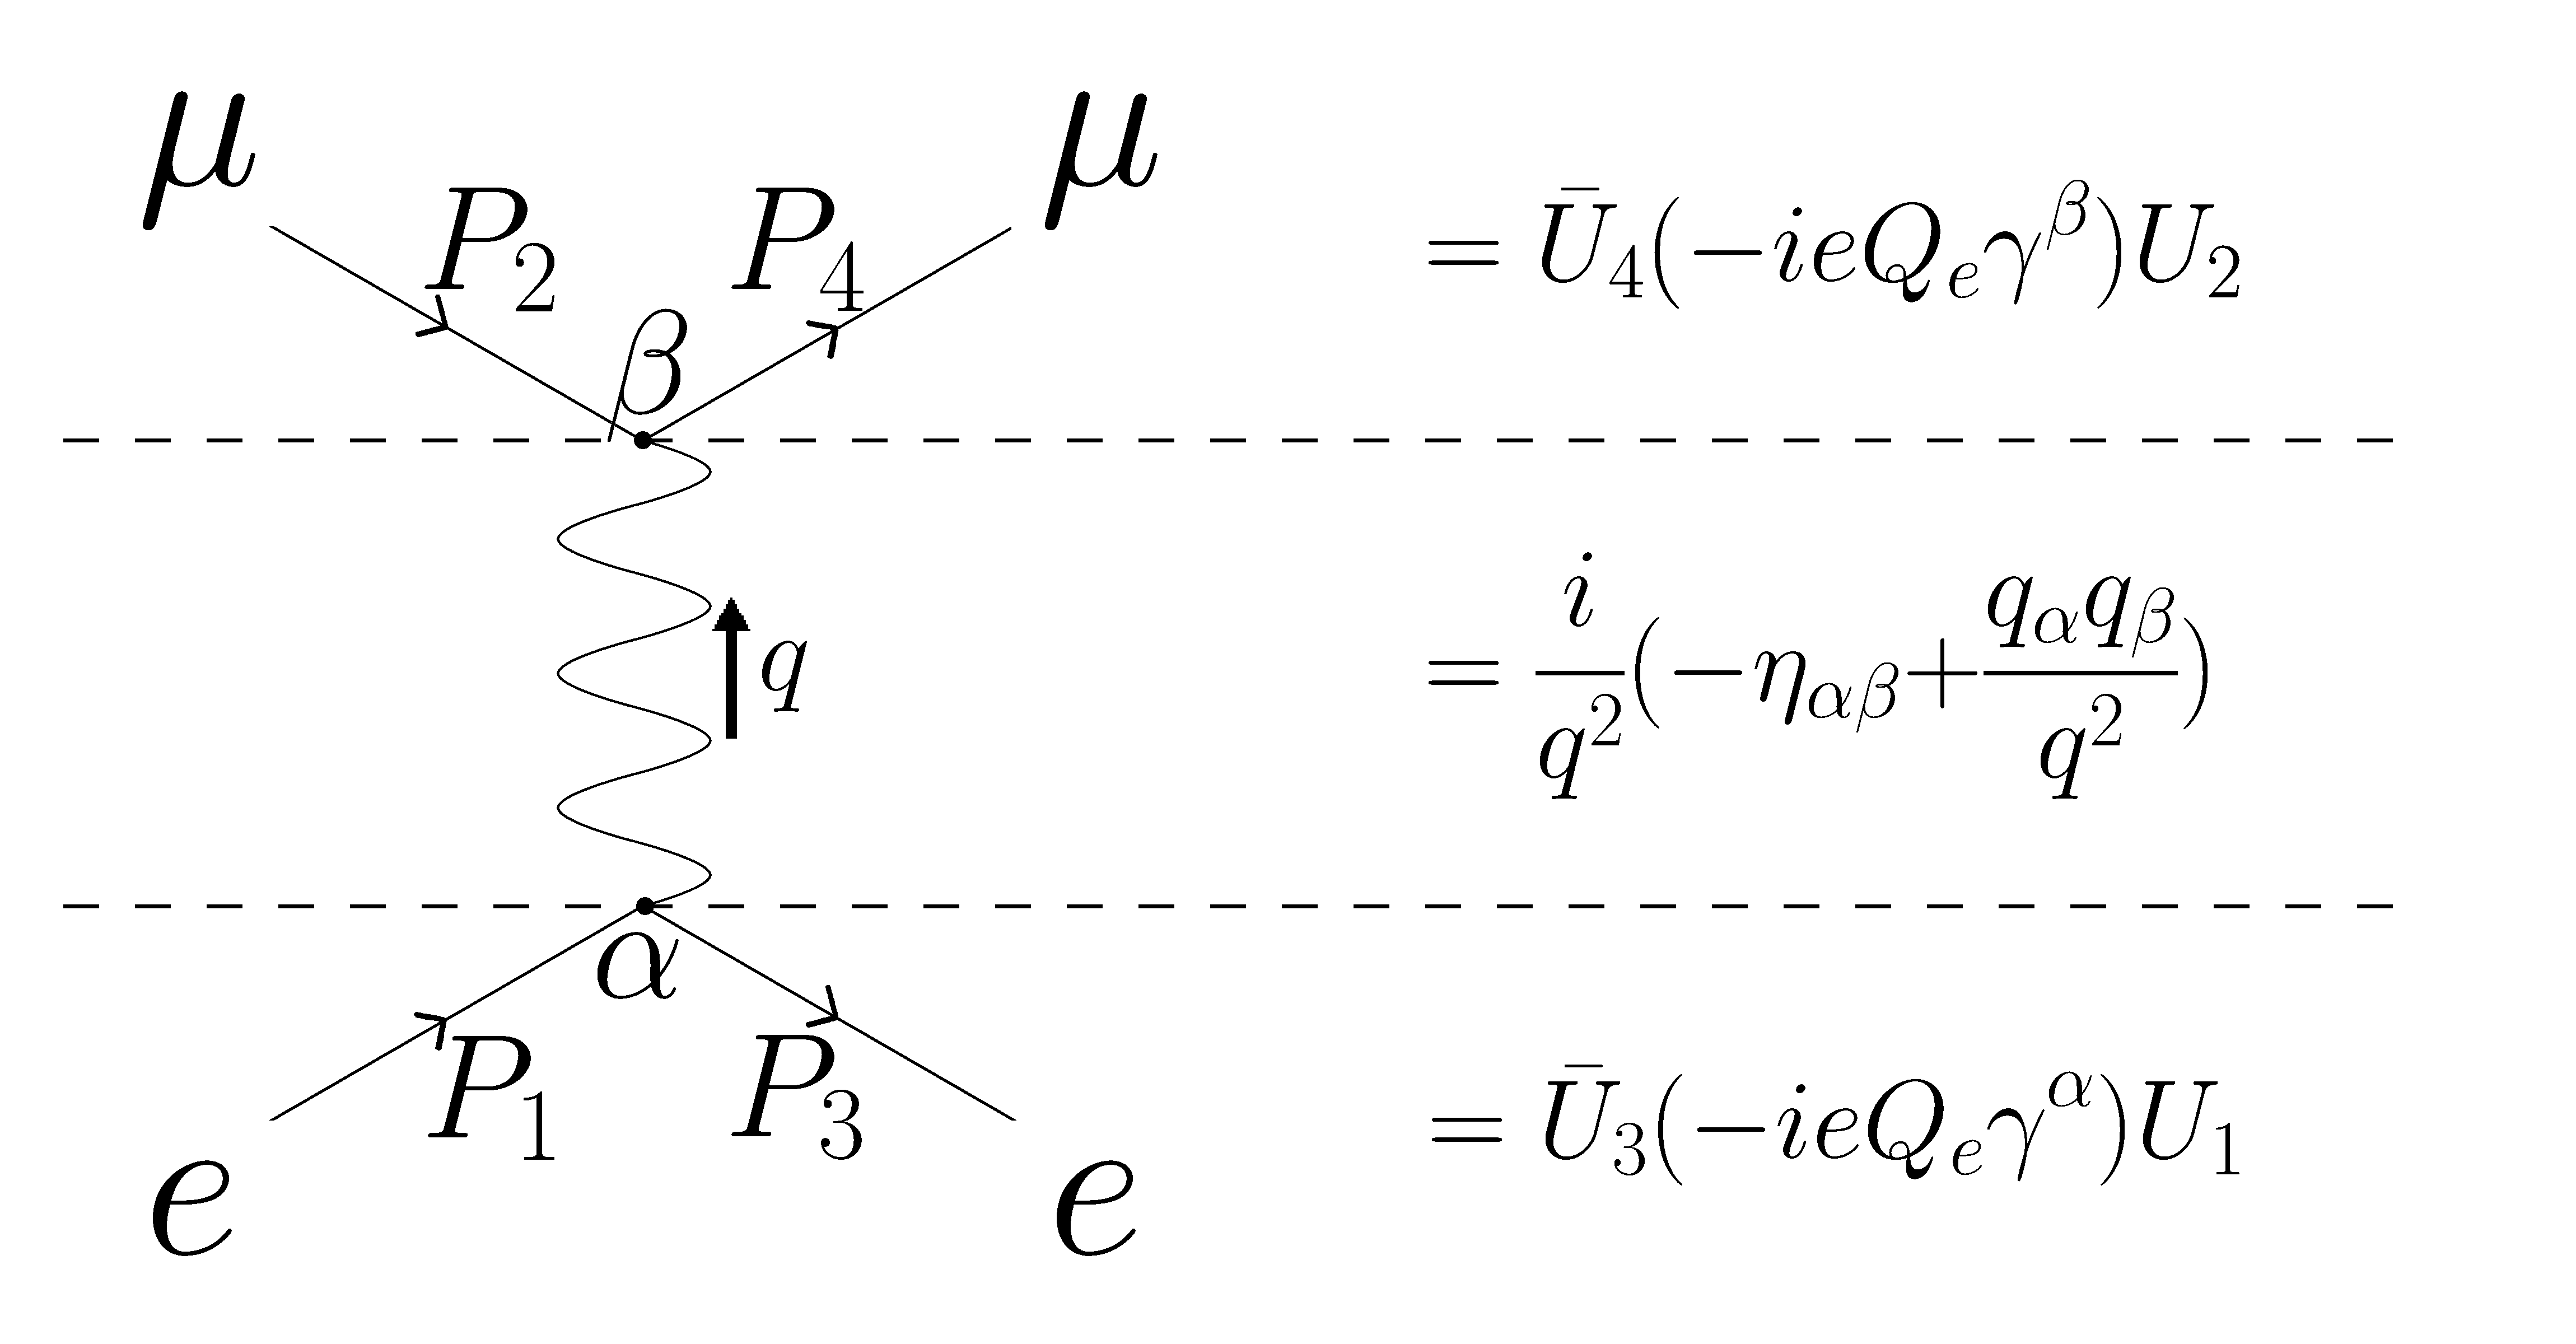
\includegraphics[width=\textwidth]{Figures/MottFeynmanMath} 
  \caption[Mathematical interpretation the three branches of the Feynman diagram in Figure~\ref{fig:mottFeynman}.]{Mathematical interpretation the three branches of the Feynman diagram in Figure~\ref{fig:mottFeynman}. The top part is the muon flow, the middle is the virtual photon, and the bottom is the electron flow.}
  \label{fig:mottFeynmanMath}
\end{figure}
Ignoring the multiplicative constants, Eq. \eqref{eqn:mottFeynmanScatteringAmplitude} can be rearragned to
\begin{align*}
\mathcal{M} \, \propto \, \bar{U}_4\gamma^\beta U_2 \, * \, \frac{1}{q^2}(-\eta_{\alpha\beta}+\frac{q_\alpha q_\beta}{q^2}) \, *\, \bar{U}_3\gamma^\alpha U_1.
\end{align*}
Note that the second term in the parenthesis (i.e. $q_\alpha q_\beta / q^2$) vanishes. To see this, observe that when the expression is multiplied out the second term $q_\alpha q_\beta / q^2$ becomes proportional to $\bar{U}_4\gamma^\beta U_2 q_\beta$. By conservation of $P_\beta$ at vertex $\beta$, it can be seen that $P_{2\beta}+q_\beta=P_{4\beta}$, or more usefully $q_\beta=P_{4\beta}-P_{2\beta}$. Then
\begin{align*}
\bar{U}_4\gamma^\beta U_2 q_\beta&= \bar{U}_4(\gamma^\beta(P_{4\beta}-P_{2\beta})) U_2\\
&= \bar{U}_4(\gamma^\beta P_{4\beta}-\gamma^\beta P_{2\beta}) U_2 .
\end{align*}
Eq. \eqref{eqn:diracEquation} states that $\gamma^\alpha P_\alpha-m=0$, and so
\begin{align*}
\bar{U}_4\gamma^\beta U_2 q_\beta &= \bar{U}_4 (m_\mu-m_\mu) U_2=0.
\end{align*}
For this reason, the second term in parenthesis vanishes entierly, leaving
\begin{align*}
\mathcal{M} \, \propto \, \bar{U}_4\gamma^\beta U_2 \, * \, \frac{\eta_{\alpha\beta}}{q^2}\, *\, \bar{U}_3\gamma^\alpha U_1.
\end{align*}
Propagating the $\eta_{\alpha\beta}$ through,
\begin{align*}
\mathcal{M} \, \propto \, \bar{U}_4\gamma^\beta U_2 \, * \, \frac{1}{q^2}\, *\, \bar{U}_3\gamma_\beta U_1.
\end{align*}
The final cross section is proportional to $|\mathcal{M}|^2$, and so
\begin{align*}
|\mathcal{M}|^2 \, \propto \, \frac{1}{q^4}\, *\, \bar{U}_4\gamma^\beta U_2 [\bar{U}_4\gamma^\delta U_2]^* \, * \,  \bar{U}_3\gamma_\beta U_1 [\bar{U}_3\gamma_\delta U_1]^*.
\end{align*}
Since $\bar{U}_4\gamma^\beta U_2$ is the same as $\bar{U}_3\gamma_\beta U_1$ except for notation, from here the quantity $\bar{U}_4\gamma^\beta U_2 [\bar{U}_4\gamma^\delta U_2]^* $ is reduced and the same treatment is applied to $\bar{U}_3\gamma_\beta U_1 [\bar{U}_3\gamma_\delta U_1]^*$.

Since $\bar{U}_4\gamma^\delta U_2 \in \mathbb{C}$ in Dirac space, 
\begin{align*}
[\bar{U}_4\gamma^\delta U_2]^*&=[\bar{U}_4\gamma^\delta U_2]^\dagger\\
&=U^\dagger _2 {\gamma^\delta}^\dagger \bar{U}_4 ^\dagger.
\end{align*}
Observe that since $\gamma^\delta$ has the form
\begin{align*}
\gamma^\delta=	\begin{pmatrix}
			A&B\\
			-B&-A
			\end{pmatrix}
\end{align*}
then
\begin{align*}
\gamma^0\gamma^\delta\gamma^0 &=	
	\begin{pmatrix}
	I_2 & 0\\
	0 & I_2
	\end{pmatrix}
	\begin{pmatrix}
	A&B\\
	-B&-A
	\end{pmatrix}
	\begin{pmatrix}
	I_2 & 0\\
	0 & I_2
	\end{pmatrix}
\\
&=	\begin{pmatrix}
	A&-B\\
	B&-A
	\end{pmatrix}
\\
&= {\gamma^\delta}^\dagger,
\end{align*}
and so
\begin{align*}
[\bar{U}_4\gamma^\delta U_2]^*=U^\dagger _2 [\gamma^0 \gamma^\delta \gamma^0] \bar{U}_4 ^\dagger.
\end{align*}
Recall the definition of the spinor adjoint in Eq. \eqref{eqn:spinorAdjoint}:
\begin{align*}
\bar{U}=U^\dagger \gamma^0.
\end{align*}
Then
\begin{align*}
\bar{U}_4 ^\dagger&=(U_4 ^\dagger \gamma^0)^\dagger\\
&={\gamma^0}^\dagger {U_4^\dagger}^\dagger\\
&=\gamma^0 U_4,
\end{align*}
which results in
\begin{align*}
[\bar{U}_4\gamma^\delta U_2]^*&=U^\dagger _2 [\gamma^0 \gamma^\delta \gamma^0] [\gamma^0 U_4],
\end{align*}
or more suggestively,
\begin{align*}
[\bar{U}_4\gamma^\delta U_2]^*&=\,[U^\dagger _2 \gamma^0] \, \gamma^\delta \, [\gamma^0 \gamma^0] \, U_4\\
&=\bar{U}_2 \gamma^\delta U_4.
\end{align*}
This results in
\begin{align} \label{eqn:mottIntermediate}
|\mathcal{M}|^2 \propto \frac{1}{q^4} \, * \, \bar{U}_4\gamma^\beta U_2 \bar{U}_2 \gamma^\delta U_4 \, * \, \bar{U}_3\gamma_\beta U_1 \bar{U}_1 \gamma_\delta U_3.
\end{align}
In principle, if the spinors of the muons were known (e.g. the muons were part of a polarized beam) this could be evaluated directly. However, in general the spinors are not known. As an approximation, it is necessary to average the spinors over their spins. Again, starting with the muons and extrapolating the treatment to the electrons,
\begin{align*}
\left< \bar{U}_4 \gamma^\beta U_2 \bar{U}_2 \gamma^\delta U_4 \right> _\text{spin 2}
&= \frac{1}{2} \sum _{s_2 = 1} ^2 \bar{U}_4 \gamma^\beta U_2 ^{(s_2)} \bar{U}_2 ^{(s_2)} \gamma^\delta U_4\\
&= \frac{1}{2} \bar{U}_4 \gamma^\beta \left[ \sum _{s_2 = 1} ^2 U_2 ^{(s_2)} \bar{U}_2 ^{(s_2)} \right] \gamma^\delta U_4.
\end{align*}
Recall the completeness property of spinors (Eq. \eqref{eqn:spinorCompleteness}):
\begin{align*}
\sum _s U^{(s)}\bar{U}^{(s)} = \gamma^\alpha P_\alpha + m.
\end{align*}
Then
\begin{align*}
\left< \bar{U}_4 \gamma^\beta U_2 \bar{U}_2 \gamma^\delta U_4 \right> _\text{spin 2}
= \frac{1}{2} \bar{U}_4 \gamma^\beta (\gamma^\epsilon P_{2\epsilon}+m_\mu)\gamma^\delta U_4.
\end{align*}
Averaging similarly over the spin for particle \#4 yields
\begin{align*}
\left< \bar{U}_4 \gamma^\beta U_2 \bar{U}_2 \gamma^\delta U_4 \right> _\text{spin 2, spin 4}
&= \frac{1}{2} \frac{1}{2} \sum_{s_4=1} ^2 \bar{U}_4 ^{(s_4)} [\gamma^\beta (\gamma^\epsilon P_{2\epsilon}+m_\mu)\gamma^\delta] U_4 ^{(s_4)}.
\end{align*}
Now, spinors do not generally commute, but their components (which are scalars) do. Observing that $\bar{U}$ is a 1x4 row vector, the bracketed term is a 4x4 matrix, and $U$ is a 4x1 column vector, it is possible to write out the matrix multiplication as an explicit double sum over the indices $i,j$:
\begin{align*}
\left< \bar{U}_4 \gamma^\beta U_2 \bar{U}_2 \gamma^\delta U_4 \right> _\text{s2, s4}
&=\frac{1}{4}\sum_{s_4=1} ^2 \sum_{i,j=1} ^4 \bar{U}_{4i} ^{(s_4)} [\gamma^\beta(\gamma^\epsilon P_{2\epsilon}+m_\mu)\gamma^\delta]_{ij} U_{4j} ^{(s_4)}\\
&=\frac{1}{4}\sum_{i,j=1} ^4 \Big([\gamma^\beta(\gamma^\epsilon P_{2\epsilon}+m_\mu)\gamma^\delta]_{ij} \Big[ \sum_{s_4=1} ^2 \bar{U}_4 ^{(s_4)} U_4 ^{(s_4)}\Big]_{ij} \Big)
\end{align*}

Spinor completeness (Eq. \eqref{eqn:spinorCompleteness}) requires a summation over $U\bar{U}$, not $\bar{U}U$. However, $\bar{U}U$ is still useful. Since $A^T+B^T=[A+B]^T$,
\begin{align*}
\sum \bar{U}U 
&= \Big[\sum (\bar{U}U)^T\Big]^T\\
&=\Big[\sum U^T \bar{U}^T\Big]^T.
\end{align*}
Again explicitly writing the matrix multiplication,
\begin{align*}
\sum \bar{U}U 
&=\Big[\sum\Big(\sum_{k,l} ^4 (U_k)^T(\bar{U}_l)^T\Big)\Big]^T\\
&=\Big[\sum_{k,l} ^4 \Big(\sum (U_k)^T (\bar{U}_l)^T \Big)\Big]^T\\
&=\Big[\sum_{k,l}^4\Big(\sum U_l \bar{U}_k\Big)\Big]^T\\
&=\Big[\sum_{k,l}^4\Big(\sum U\bar{U})_{l,k}\Big]^T.
\end{align*}
Now it is possible to use spinor completeness (Eq. \eqref{eqn:spinorCompleteness}):
\begin{align*}
\sum \bar{U}U 
&=\Big[\sum_{k,l}\big(\gamma^\alpha P_alpha + m\big) _{l,k}\\
&=(\gamma^\alpha P_\alpha + m)^T.
\end{align*}
Conclusively, if the $i$-$j^{th}$ component of $\sum \bar{U}U$ is desired, then the indices of Eq. \eqref{eqn:spinorCompleteness} must be exchanged:
\begin{align*}
\Big[\sum\bar{U} U\Big]_{i,j}
&=[(\gamma^\alpha P_\alpha + m)^T]_{i,j}\\
&=[(\gamma^\alpha P_\alpha + m)_{i,j}]^T\\
&=[\gamma^\alpha P_\alpha + m]_{j,i}.
\end{align*}
This results in
\begin{align*}
\left< \bar{U}_4 \gamma^\beta U_2 \bar{U}_2 \gamma^\delta U_4 \right> _\text{s2, s4}
&=\frac{1}{4}\sum_{i,j=1} ^4 \Big([\gamma^\beta(\gamma^\epsilon P_{2\epsilon}+m_\mu)\gamma^\delta]_{ij} [\gamma^\kappa P_{4\kappa}+m_\mu]_{j,i} \Big).
\end{align*}
Upon the concatenation of the subscripts $i,j$ and $j,i$, it can be seen that
\begin{align*}
\left< \bar{U}_4 \gamma^\beta U_2 \bar{U}_2 \gamma^\delta U_4 \right> _\text{s2, s4}
&=\frac{1}{4}\sum_{i=1} ^4 \Big([\gamma^\beta(\gamma^\epsilon P_{2\epsilon}+m_\mu)\gamma^\delta] (\gamma^\kappa P_{4\kappa}+m_\mu) \Big)_{ii}.
\end{align*}
This is now the definition of a trace ($\sum_i M_{ii} \equiv \text{Tr} (M)$). Then
\begin{align*}
\left< \bar{U}_4 \gamma^\beta U_2 \bar{U}_2 \gamma^\delta U_4 \right> _\text{s2, s4}
&=\frac{1}{4}\text{Tr}[\gamma^\beta(\gamma^\epsilon P_{2\epsilon}+m_\mu)\gamma^\delta (\gamma^\kappa P_{4\kappa}+m_\mu)].
\end{align*}
Using the addition property of traces, it is clear that there are four terms to evaluate:
\begin{align*}
i) &\quad \text{Tr}(\gamma^\beta \gamma^\epsilon P_{2\epsilon}\gamma^\delta\gamma^\kappa P_{4\kappa})\\
ii) &\quad \text{Tr}(\gamma^\beta \gamma^\epsilon P_{2\epsilon}\gamma^\delta m_\mu)\\
iii) &\quad \text{Tr}(\gamma^\beta m_\mu \gamma^\delta\gamma^\kappa P_{4\kappa})\\
iv) &\quad \text{Tr}(\gamma^\beta m_\mu \gamma^\delta m_\mu).
\end{align*}
The derivations for the solutions to these traces can be found in Appendix~\ref{apx:gammaMatrixProofs}. The first term is the trace of four $\gamma$ matrices and can be solved by using Eq. \eqref{eqn:griffithsRule13}:
\begin{align*}
\text{Tr}(\gamma^\beta \gamma^\epsilon P_{2\epsilon}\gamma^\delta\gamma^\kappa P_{4\kappa})
&= P_{2\epsilon}P_{4\kappa}\text{Tr}(\gamma^\beta \gamma^\epsilon\gamma^\delta\gamma^\kappa)\\
&=4P_{2\epsilon} P_{4\kappa} (\eta^{\beta\epsilon}\eta^{\delta\kappa}-\eta^{\beta\delta}\eta^{\epsilon\kappa}+\eta^{\beta\kappa}\eta^{\epsilon\delta})\\
&=4(P_2 ^\beta P_4 ^\delta - P_2 \cdot P_4 \eta^{\beta\delta} + P_2 ^\delta P_4 ^\beta).
\end{align*}
The second term is the trace of an odd number of $\gamma$ matrices, and is equal to zero via Eq. \eqref{eqn:griffithsRule10}:
\begin{align*}
\text{Tr}(\gamma^\beta \gamma^\epsilon P_{2\epsilon}\gamma^\delta m_\mu)
&= P_{2\epsilon}m_\mu\text{Tr}(\gamma^\beta \gamma^\epsilon\gamma^\delta)\\
&=0.
\end{align*}
The third term is also a trace of an odd number of $\gamma$ matrices:
\begin{align*}
\text{Tr}(\gamma^\beta m_\mu \gamma^\delta\gamma^\kappa P_{4\kappa})
&=m_\mu P_{4\kappa} \text{Tr}(\gamma^\beta  \gamma^\delta\gamma^\kappa)\\
&=0.
\end{align*}
The final term is the trace of two $\gamma$ matrices, and results in the Minkowski metric via Eq. \eqref{eqn:griffithsRule12}:
\begin{align*}
\text{Tr}(\gamma^\beta m_\mu \gamma^\delta m_\mu)
&=m_\mu ^2 \text{Tr}(\gamma^\beta \gamma^\delta)\\
&=4 m_\mu ^2 \eta^{\beta\delta}.
\end{align*}
Putting it all together results in
\begin{align*}
\left< \bar{U}_4 \gamma^\beta U_2 \bar{U}_2 \gamma^\delta U_4 \right> _\text{s2, s4}
&=P_2^\beta P_4^\delta - P_2 \cdot P_4 \eta^{\beta\delta}+P_2 ^\delta P_4 ^\beta + m_\mu ^2 \eta^{\beta\delta}.
\end{align*}

The electron portion is mathematically the same. Symbolically, contravariant indices become covariant (e.g. $\gamma^\beta$ becomes $\gamma_\beta$), the mass is now the electron mass (i.e. $m_\mu$ becomes $m_e$), and the even subscripts become odd (i.e. $P_2$, $P_4$ become $P_1$, $P_3$). Explicitly, Eq. \eqref{eqn:mottIntermediate} becomes
\begin{align*}
\left< |\mathcal{M}|^2\right>
\propto\frac{1}{q^4} \, * \, &\left< \bar{U}_4 \gamma^\beta U_2 \bar{U}_2 \gamma^\delta U_4 \right> _\text{s2, s4} \, * \, \left< \bar{U}_3 \gamma_\beta U_1 \bar{U}_1 \gamma_\delta U_4 \right> _\text{s1, s3}\\
\propto \frac{1}{q^4} \, * \, &(P_2^\beta P_4^\delta - P_2 \cdot P_4 \eta^{\beta\delta}+P_2 ^\delta P_4 ^\beta + m_\mu ^2 \eta^{\beta\delta}) \, * \\
&(P_{1\beta} P_{3\delta} - P_1 \cdot P_3 \eta_{\beta\delta}+P_{1\delta} P_{3\beta} + m_e ^2 \eta_{\beta\delta}).
\end{align*}
Explicitly, the algebra is
\begin{align*}
\left< |\mathcal{M}|^2\right> \propto
\frac{1}{q^4} \, * \, [ &(P_1 \cdot P_2)(P_3 \cdot P_4)-(P_1\cdot P_3)(P_2 \cdot P_4) + (P_1 \cdot P_4)(P_2\cdot P_3)+\\
&m_e ^2 (P_2 \cdot P_4)-(P_1\cdot P_3)(P_2\cdot P_4)+4(P_1\cdot P_3)(P_2\cdot P_4)-\\
&(P_1\cdot P_3)(P_2\cdot P_4) - 4m_e ^2 (P_2 \cdot P_4)+(P_1\cdot P_4)(P_2 \cdot P_3)-\\
&(P_1 \cdot P_3)(P_2 \cdot P_4) + (P_1 \cdot P_2) (P_3 \cdot P_4) + m_e ^2 (P_2 \cdot P_4)+\\
&m_\mu ^2 (P_1 \cdot P_3)-4m_\mu ^2 (P_1\cdot P_3) + m_\mu ^2 (P_1 \cdot P_3) + 4m_\mu ^2 m_e ^2],
\end{align*}
with $\eta^{\alpha\beta} \eta_{\alpha\beta} = 4$. Gathering the like terms, this reduces to
\begin{align*}
\left< |\mathcal{M}|^2\right> \propto \frac{1}{q^4} [&2(P_1 \cdot P_4)(P_2\cdot P_3)+2(P_1\cdot P_2)(P_3 \cdot P_4) - \\
&2 m_e ^2 (P_2 \cdot P_4)-2m_\mu ^2 (P_1 \cdot P_3) + 4 m_\mu ^2 m_e ^2 ].
\end{align*}
Up until here, this is a quite general experession for two particles interacting via virtual photon exchange. For COSY, straggling and scattering are mutually exclusive processes: first the straggling routine is called and then the scattering routine is called. Therefore, for this model it must be assumed that there is no energy exchange between the muon and electron. Consequently, since the electron is bound it remains fixed and the muon scatters. This can be seen diagrammatically in Figure~\ref{fig:mottScattering}.

\begin{figure}
  \centering
    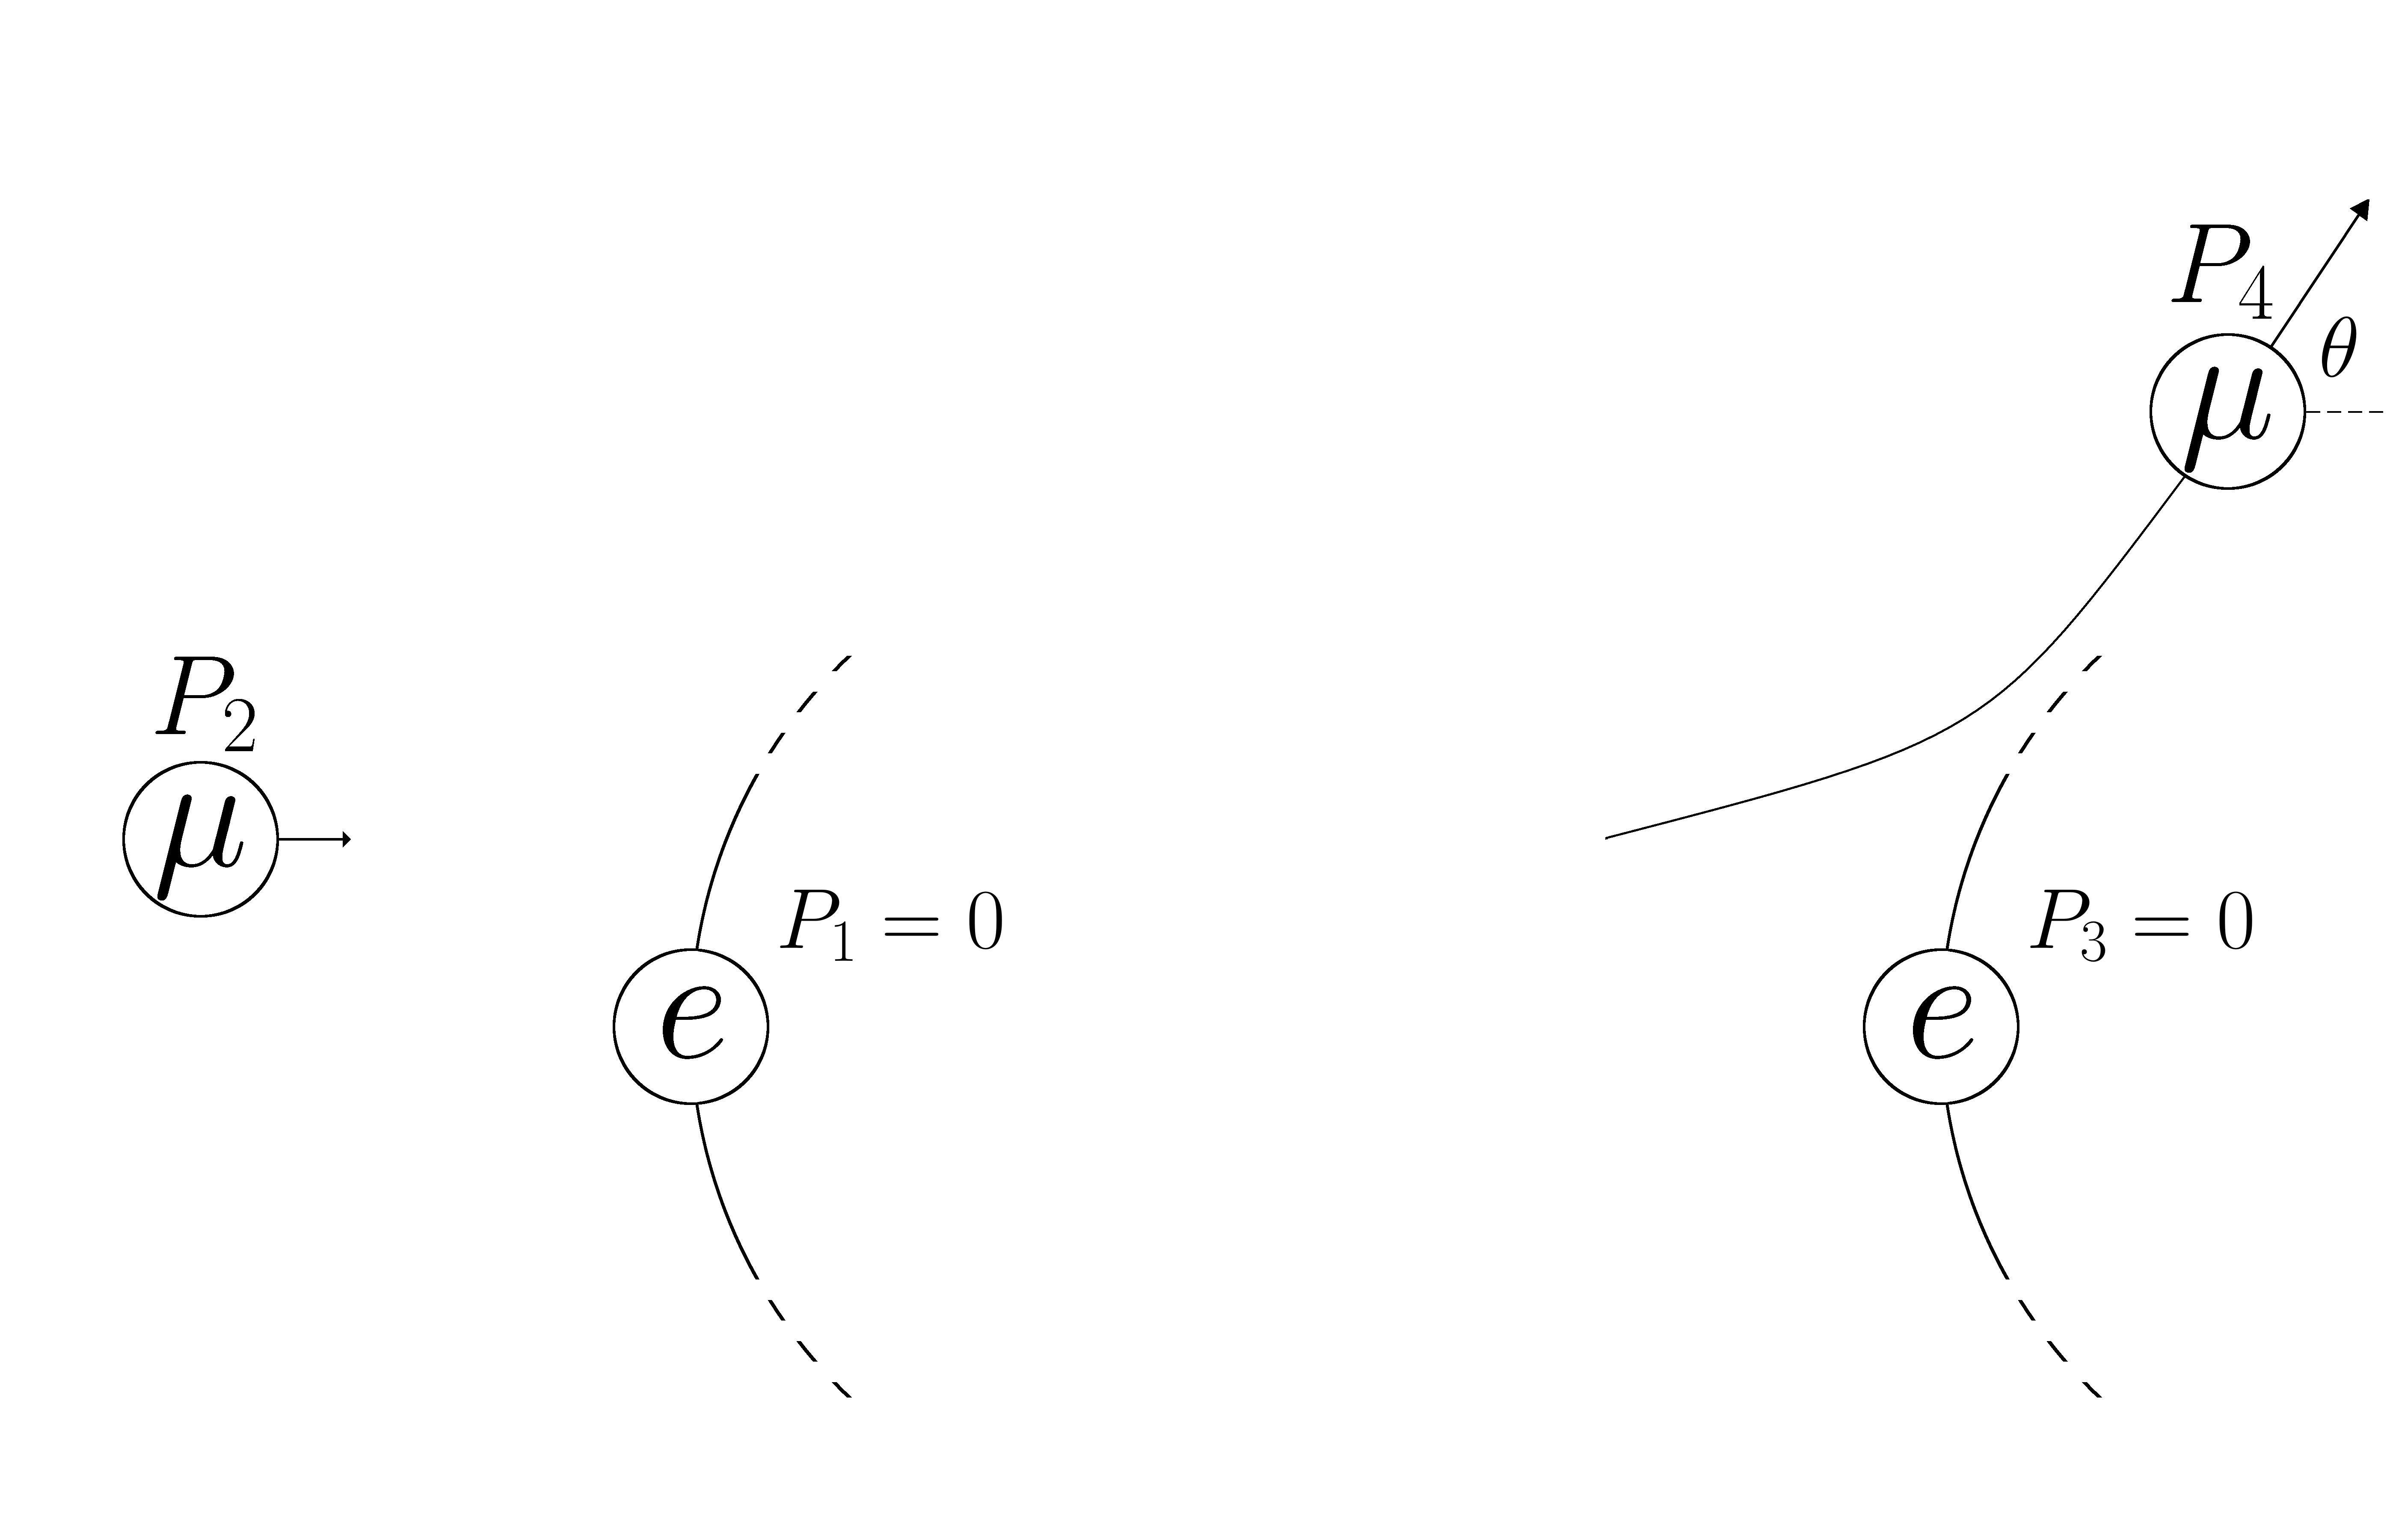
\includegraphics[width=\textwidth]{Figures/MottScattering} 
  \caption[COSY treatment of muon-electron scattering.]{COSY treatment of muon-electron scattering. Since the routines are called separately, the model assumes no straggling while scattering.}
  \label{fig:mottScattering}
\end{figure}

Now it is clear that $P_1=P_3=(m_e, 0, 0, 0)$. Furthermore, since the total energy of the muon is conserved $E_2 = E_4 = E_\mu$ and $P_2 = (E_\mu, \vec{p}_2)$ and $P_4 = (E_\mu \vec{p}_4)$ and so
\begin{align*}
P_1 \cdot P_2 &= E_\mu m_e &\qquad P_1 \cdot P_3 &= m_e ^2 \\
P_1 \cdot P_4 &= E_\mu m_e &\qquad  P_2 \cdot P_3 &= E_\mu m_e \\
P_2 \cdot P_4 &= E_\mu ^2 - \vec{p}_2 \cdot \vec{p}_4 &\qquad = E_\mu ^2  & - p_\mu ^2 \cos\theta\\
P_3 \cdot P_4 &= E_\mu m_e.
\end{align*}
Then
\begin{align*}
\left< |\mathcal{M}|^2\right> \propto \frac{1}{q^4} [2 (E_\mu m_e)(E_\mu m_e) + 2 (E_\mu m_e) (E_\mu m_e) - 2 m_e ^2 (E_\mu^2 - p_\mu ^2 \cos\theta) - 2 m_\mu ^2 m_e ^2 + 4 m_\mu ^2 m_e ^2 ].
\end{align*}
Factoring out the term $2m_e ^2$, 
\begin{align*}
\left< |\mathcal{M}|^2\right> 
&\propto \frac{1}{q^4} (E_\mu ^2 + E_\mu ^2 - E_\mu ^2 + p_\mu ^2 \cos\theta - m_\mu ^2+ 2 m_\mu ^2 ) \\
&\propto \frac{1}{q^4} (E_\mu ^2 + p_\mu \cos\theta + m_\mu^2)\\
&\propto \frac{1}{q^4} (p_\mu + m_\mu + p_\mu \cos\theta + m_\mu^2)\\
&\propto \frac{1}{q^4} (2 m_\mu ^2 + p_\mu (1+\cos\theta)).
\end{align*}
Factoring out $2m_\mu ^2$ and observing that $p/m = \beta\gamma$ yields
\begin{align*}
\left< |\mathcal{M}|^2\right> 
&\propto \frac{1+\frac{(\beta\gamma)^2}{2} (1+\cos\theta)  }{q^4}.
\end{align*}
Again using conservation of $P_\beta$ at vertex $\beta$, it can be seen that 
\begin{align*}
P_{2\beta}+q_\beta=P_{4\beta} \quad \rightarrow \quad & q_\beta = P_{4\beta} - P_{2\beta}
\end{align*}.
Then
\begin{align*}
q^2 &= ( P_{4\beta} - P_{2\beta}) ^2\\
&= ( (E_4, \vec{p}_4) - (E_2, \vec{p}_2 ) )^2\\
& = ((0, \vec{p}_4 - \vec{p}_2))^2\\
& = - (p_4 ^2 + p_2 ^2 - p_4 p_2 \cos\theta)\\
&=-2p_\mu (1-\cos\theta).
\end{align*}
Squaring $q^2$ and throwing out the constant $p_\mu$,
\begin{align*}
\left< |\mathcal{M}|^2\right> \propto \frac{1+\frac{(\beta\gamma)^2}{2} (1+\cos\theta)  }{(1-\cos\theta)^2}.
\end{align*}
Finally, the Mott cross section is obtained:
\begin{equation}\label{eqn:MottCrossSection_apx}
\frac{d\sigma}{d\Omega} \propto \frac{1+\frac{(\beta\gamma)^2}{2} (1+\cos\theta)  }{(1-\cos\theta)^2}.
\end{equation}
Observe that for a non-relativistic beam of muons, $\beta\gamma \rightarrow 0$ and this reduces to the Rutherford cross section (Eq. \eqref{eqn:rutherford}).
%-------------------------------------------------------------------------------
\Appendix{A Brief Review of Relevant Particle Physics} \label{apx:particlePhysicsReview}

Since this dissertation concerns only muons interacting with electrons, this
brief review only covers particles with spin 1/2. This review follows
\cite{griffithspp}.
Particles of four-momentum $P=(E, \vec{p})=(E,p_x,p_y,p_z)$ must satisfy the
relativistic
energy-momentum relation:

\begin{gather} \label{eqn:energyMomentumRelation}
P^{\alpha}P_\alpha - m^2 = 0,
\end{gather}
since
\begin{align*}
P^{\alpha}P_\alpha - m^2&=E^2-p^2-m^2 \\ &=E^2-(p^2+m^2) \\ &=E^2-E^2=0.
\end{align*}

For particles at rest (i.e. $\vec{p}=0$), this can be written as:
\begin{align*}
P^\alpha P_\alpha - m^2 = (p^0+m)(p^0-m)=0,
\end{align*}
and so clearly the energy $p^0=E$ has to be either the rest mass or the negative
of the rest mass
(for antiparticles). However, for particles which are not at rest, if this same
form is desired
then it should look something like
\begin{align*}
P^\alpha P_\alpha - m^2 &= (\gamma^\beta P_\beta + m)(\gamma^\delta P_\delta
-m).
\end{align*}
One may solve this equation for the coefficients
$\gamma^\beta=(\gamma^0,\gamma^1,\gamma^2,\gamma^3)$, but no scalars solve this
complex system.
Dirac proposed that the various $\gamma$s were actually matrices, not scalars.
This approach has the solution:
\begin{align*}
\gamma^0=
\begin{pmatrix}
I_2 & 0\\
0 & -I_2
\end{pmatrix} \qquad \gamma^j=
\begin{pmatrix}
0 & \sigma^j\\
-\sigma^j & 0
\end{pmatrix},
\end{align*}
where $\sigma^j$ are the Pauli matrices. This leads to the Dirac equation for
particles (for
antiparticles, simply switch the sign of the mass):
\begin{equation}\label{eqn:diracEquation}
\gamma^\alpha P_\alpha - m = 0.
\end{equation}

These particles can be represented by the wavefunctions for free particles,
\begin{gather*}
\psi(x)=Ce^{-(i/\hbar)p\cdot x} U^{(s)} (P),
\end{gather*}
where $C$ is some amplitude, $U$ is the spinor, and $s$ is the spin state of the
particle (in this
case $s=1,2$). Antiparticle spinors are represented by $V$ (unused in this work).
Spinor adjoints are defined by
\begin{equation}\label{eqn:spinorAdjoint}
\bar{U}=U^\dagger\gamma^0={U^*}^T \gamma^0,
\end{equation}
where $^*$ represents the complex conjugate and $^T$ the transpose. These
spinors satisfy the Diracequation:
\begin{align*}
(\gamma^\alpha P_\alpha - m)U=0,
\end{align*}
they are orthogonal:
\begin{align*}
\bar{U}^{(1)}U^{(2)}=0,
\end{align*}
and they are normalized:
\begin{align*}
\bar{U}U=2m,
\end{align*}
and they are complete:
\begin{equation}\label{eqn:spinorCompleteness}
\sum_{s=1}^2 U^{(s)}\bar{U}^{(s)}=(\gamma^\alpha P_\alpha + m).
\end{equation}
These spinors are four-component column vectors, and spinors describing particles ($U$) and antiparticles ($V$) for spin 1/2 particles could be represented as, for instance
\begin{align*}
U^{(1)}=
	\begin{pmatrix}
	1\\0\\0\\0
	\end{pmatrix}
&\qquad
U^{(2)}=
	\begin{pmatrix}
	0\\1\\0\\0
	\end{pmatrix}
\\
V^{(1)}=
	\begin{pmatrix}
	0\\0\\1\\0
	\end{pmatrix}
&\qquad
V^{(2)}=
	\begin{pmatrix}
	0\\0\\0\\1
	\end{pmatrix},
\end{align*}
but are usually more complicated if unpolarized.

%-------------------------------------------------------------------------------
\Appendix{Explicit Forms of the Dirac Gamma Matrices and Pauli Matrices}\label{apx:explicitMatrices}

From the conventions in \cite{griffithspp}
it is observed that
the Pauli matrices are defined as:

\begin{align*}
\sigma^1=
\begin{pmatrix}
0 & 1\\
1 & 0
\end{pmatrix}
\qquad
\sigma^2=
\begin{pmatrix}
0 & -i\\
i & 0
\end{pmatrix}
\qquad
\sigma^3=
\begin{pmatrix}
1 & 0\\
0 & -1
\end{pmatrix}
.
\end{align*}

Then the Dirac matrices follow as:
\begin{equation} \label{eqn:gammaExplicit}
\begin{split}
\gamma^0=
\begin{pmatrix}
1 & 0 & 0 & 0\\
0 & 1 & 0 & 0 \\
0 & 0 & -1 & 0 \\
0 & 0 & 0 & -1
\end{pmatrix}
& \qquad \gamma^1 =
\begin{pmatrix}
0 & 0 & 0 & 1\\
0 & 0 & 1 & 0 \\
0 & -1 & 0 & 0 \\
-1 & 0 & 0 & 0
\end{pmatrix}
\\
\gamma^2=
\begin{pmatrix}
0 & 0 & 0 & -i\\
0 & 0 & i & 0 \\
0 & i & 0 & 0 \\
-i & 0 & 0 & 0
\end{pmatrix}
& \qquad \gamma^3 =
\begin{pmatrix}
0 & 0 & 1 & 0\\
0 & 0 & 0 & -1 \\
-1 & 0 & 0 & 0 \\
0 & 1 & 0 & 0
\end{pmatrix}
.
\end{split}
\end{equation}
%-------------------------------------------------------------------------------
\Appendix{Proofs of Useful Dirac Gamma Matrix Trace Identities}
\label{apx:gammaMatrixProofs}

\Section{Proof of $(\gamma^5)^2=I_4$} \label{ssc:gamma52}

Let $\gamma^5\equiv i\gamma^0 \gamma^1 \gamma^2 \gamma^3$. Then explicitly
carrying out the
multiplication yields
\begin{align} \nonumber
\gamma^5&=i
\begin{pmatrix}
0 & 0 & 0 & 1\\
0 & 0 & 1 & 0\\
0 & 1 & 0 & 0\\
1 & 0 & 0 & 0
\end{pmatrix}
\cdot -i
\begin{pmatrix}
0 & 1 & 0 & 0\\
1 & 0 & 0 & 0\\
0 & 0 & 0 & 1\\
0 & 0 & 1 & 0
\end{pmatrix}
\\ \label{eqn:gamma5}
\gamma^5 &= \ \,
\begin{pmatrix}
0 & 0 & 1 & 0\\
0 & 0 & 0 & 1\\
1 & 0 & 0 & 0 \\
0 & 1 & 0 & 0
\end{pmatrix}.
\end{align}
Then
\begin{equation}\label{eqn:gamma52}
(\gamma^5)^2=I_4.
\end{equation}

\Section{Proof of $\gamma^5\gamma^\alpha=-\gamma^\alpha\gamma^5$}
\label{ssc:gamma5Anticommutator}

Let the form of $\gamma^\alpha$ be represented as
\begin{align*}
\begin{pmatrix}
A & B\\
-B & -A
\end{pmatrix}
\end{align*}
(i.e. for $\alpha=0$, $A=I_2$ and $B=0$; otherwise $A=0$ and $B=\sigma^\alpha$).
Then using the
explicit form of $\gamma^5$ in Eq. \eqref{eqn:gamma5}:
\begin{align*}
\begin{pmatrix}
0 & I_2\\
I_2 & 0
\end{pmatrix}
\begin{pmatrix}
A & B\\
-B & -A
\end{pmatrix}
+
\begin{pmatrix}
A & B\\
-B & -A
\end{pmatrix}
\begin{pmatrix}
0 & I_2\\
I_2 & 0
\end{pmatrix}
=
\begin{pmatrix}
0 & 0\\
0 & 0
\end{pmatrix}
.
\end{align*}
Therefore, 
\begin{equation}\label{eqn:gamma5Anticommutator}
\gamma^5 \gamma^\alpha=-\gamma^\alpha \gamma^5.
\end{equation}

\Section{Proof of Tr(\textit{odd number of $\gamma$ matrices}) = 0}
\label{ssc:gammaOdd=0}

Let there be the trace of an arbitrary odd number of $\gamma$ matrices
\begin{align*}
\text{Tr}(\gamma^{\alpha_1} \gamma^{\alpha_2} ... \gamma^{\alpha_n}),
\end{align*}
such that $n$ is odd. Now insert into the beginning of the trace $\gamma^5
\gamma^5$,
\begin{align*}
\text{Tr}(\gamma^5 \gamma^5 \gamma^{\alpha_1} \gamma^{\alpha_2} ... \gamma^{\alpha_n}),\end{align*}
and there are two cases. The first makes use of $(\gamma^5)^2=I_4$ (Eqn.
\ref{eqn:gamma52}), and
results in
\begin{align}\nonumber
\text{Tr}(\gamma^5 \gamma^5 \gamma^{\alpha_1} \gamma^{\alpha_2} ...
\gamma^{\alpha_n})&=\text{Tr}(I_4
\gamma^{\alpha_1} \gamma^{\alpha_2} ... \gamma^{\alpha_n})\\
\text{Tr}(\gamma^5 \gamma^5 \gamma^{\alpha_1} \gamma^{\alpha_2} ...
\gamma^{\alpha_n})&=\text{Tr}(\gamma^{\alpha_1} \gamma^{\alpha_2} ...
\gamma^{\alpha_n})
\label{eqn:traceOdd1}
\end{align}
The next case uses the cyclic property of traces, which is
$\text{Tr}(ABCD)=\text{Tr}(BCDA)=\text{Tr}(CDAB)=\ldots$ .
Then
\begin{align*}
\text{Tr}(\gamma^5 \gamma^5 \gamma^{\alpha_1} \gamma^{\alpha_2} ...
\gamma^{\alpha_n})&=\text{Tr}(\gamma^5
\gamma^{\alpha_1} \gamma^{\alpha_2} ... \gamma^{\alpha_n}\gamma^5).
\end{align*}
Now using $\gamma^5\gamma^\alpha = -\gamma^\alpha \gamma^5$ (Eqn.
\ref{eqn:gamma5Anticommutator}):
\begin{align*}
\text{Tr}(\gamma^5 \gamma^5 \gamma^{\alpha_1} \gamma^{\alpha_2} ...
\gamma^{\alpha_n})&=\text{Tr}(\gamma^5
\gamma^{\alpha_1} \gamma^{\alpha_2} ... \gamma^5 \gamma^{\alpha_n})(-1)^1.
\end{align*}
Applying this $n$ times yields
\begin{align*}
\text{Tr}(\gamma^5 \gamma^5 \gamma^{\alpha_1} \gamma^{\alpha_2} ...
\gamma^{\alpha_n})&=\text{Tr}(\gamma^5
\gamma^5 \gamma^{\alpha_1} \gamma^{\alpha_2} ... \gamma^{\alpha_n})(-1)^n.
\end{align*}
Since $n$ is negative, $(-1)^n=-1$. Again using $(\gamma^5)^2=I_4$ (Eqn.
\ref{eqn:gamma52}), this
yields
\begin{equation}\label{eqn:traceOdd2}
\text{Tr}(\gamma^5 \gamma^5 \gamma^{\alpha_1} \gamma^{\alpha_2} ...
\gamma^{\alpha_n})=-\text{Tr}(\gamma^{\alpha_1} \gamma^{\alpha_2} ...
\gamma^{\alpha_n}).
\end{equation}
Combining Eqns. \ref{eqn:traceOdd1} and \ref{eqn:traceOdd2}:
\begin{align*}
\text{Tr}(\gamma^5 \gamma^5 \gamma^{\alpha_1} \gamma^{\alpha_2} ...
\gamma^{\alpha_n})&=\text{Tr}(\gamma^{\alpha_1} \gamma^{\alpha_2} ...
\gamma^{\alpha_n})
\\
\text{Tr}(\gamma^5 \gamma^5 \gamma^{\alpha_1} \gamma^{\alpha_2} ...
\gamma^{\alpha_n})&=-\text{Tr}(\gamma^{\alpha_1} \gamma^{\alpha_2} ...
\gamma^{\alpha_n}).
\end{align*}
Since this trace is both positive and negative the only conclusion is that it
must be zero:
\begin{align}\label{eqn:griffithsRule10}
\text{Tr}(\gamma^{\alpha_1} \gamma^{\alpha_2} ... \gamma^{\alpha_n})=0 \qquad \text{for
odd $n$.}
\end{align}

\Section{Proof of \text{Tr}($\gamma^\alpha \gamma^\beta$) = $4\eta^{\alpha\beta}$}
\label{ssc:griffithsRule12}

$\eta^{\alpha\beta}$ is an element of the Minkowski metric, which is defined here as
\begin{align*}
\eta=
\begin{pmatrix}
1 & 0 & 0 & 0 \\
0 & -1 & 0 & 0\\
0 & 0 & -1 & 0\\
0 & 0 & 0 & -1
\end{pmatrix}.
\end{align*}
Unlike $\gamma^\alpha$, $\eta^{\alpha\beta}$ is simply a number. For example, if
$\alpha\neq\beta$
then $\eta^{\alpha\beta}=0$, if $\alpha=\beta=0$ then $\eta^{\alpha\beta}=1$, and so
on. While it can be
shown explicitly, it is treated as fact that the defining algebra is
\begin{equation}\label{eqn:cliffordAlgebra}
\gamma^\alpha\gamma^\beta + \gamma^\beta \gamma^\alpha=2\eta^{\alpha\beta}I_4,
\end{equation}
which is simply to say that 
\begin{align*}
(\gamma^0)^2&=I_4\\
(\gamma^{1,2, \text{ or }3})^2&=-I_4\\
\gamma^\alpha\gamma^\beta&=0 \qquad \text{for }\alpha\neq\beta.
\end{align*}

Now, concerning the problem at hand
\begin{align*}
\text{Tr}(\gamma^\alpha \gamma^\beta)=\frac{1}{2}(\text{Tr}(\gamma^\alpha
\gamma^\beta)+\text{Tr}(\gamma^\alpha
\gamma^\beta)).
\end{align*}
Using first the cyclic property of traces, the addition of two traces, and the
defining algebra
(Eq. \eqref{eqn:cliffordAlgebra})
\begin{align*}
\text{Tr}(\gamma^\alpha
\gamma^\beta)&=\frac{1}{2}(\text{Tr}(\gamma^\alpha\gamma^\beta)+\text{Tr}(\gamma^\beta\gamma^\alpha))\\
&=\frac{1}{2}\text{Tr}(\gamma^\alpha\gamma^\beta+\gamma^\beta\gamma^\alpha)\\
&=\frac{1}{2}\text{Tr}(2\eta^{\alpha\beta}I_4).
\end{align*}
Finally,
\begin{equation}\label{eqn:griffithsRule12}
\text{Tr}(\gamma^\alpha\gamma^\beta)=4\eta^{\alpha\beta}.
\end{equation}

\Section{Proof of Tr($\gamma^\alpha\gamma^\beta\gamma^\delta\gamma^\epsilon$)
=
4($\eta^{\alpha\beta}\eta^{\delta\epsilon}-\eta^{\alpha\delta}\eta^{\beta\epsilon}+\eta^{\alpha\epsilon}\eta^{\beta\delta}$)}

Using the defining algebra (Eq. \eqref{eqn:cliffordAlgebra}), commuting $\alpha$ and $\beta$ yields
that
\begin{align*}
\text{Tr}(\gamma^\alpha\gamma^\beta\gamma^\delta\gamma^\epsilon)&=\text{Tr}((2\eta^{\alpha\beta}-\gamma^\beta\gamma^\alpha)\gamma^\delta\gamma^\epsilon)\\
&=\text{Tr}(2\eta^{\alpha\beta}\gamma^\delta\gamma^\epsilon-\gamma^\beta\gamma^\alpha\gamma^\delta\gamma^\epsilon).
\end{align*}
Using the same method first for $\alpha$ and $\delta$ and then $\alpha$ and $\epsilon$,
\begin{align*}
\text{Tr}(\gamma^\alpha\gamma^\beta\gamma^\delta\gamma^\epsilon)
&=\text{Tr}(2\eta^{\alpha\beta}\gamma^\delta\gamma^\epsilon-\gamma^\beta(2\eta^{\alpha\delta}-\gamma^\delta\gamma^\alpha)\gamma^\epsilon)\\
&=\text{Tr}(2\eta^{\alpha\beta}\gamma^\delta\gamma^\epsilon-2\eta^{\alpha\delta}\gamma^\beta\gamma^\epsilon+\gamma^\beta\gamma^\delta\gamma^\alpha\gamma^\epsilon)\\
&=\text{Tr}(2\eta^{\alpha\beta}\gamma^\delta\gamma^\epsilon-2\eta^{\alpha\delta}\gamma^\beta\gamma^\epsilon+\gamma^\beta\gamma^\delta(2\eta^{\alpha\epsilon}-\gamma^\beta\gamma^\delta\gamma^\epsilon\gamma^\alpha))\\
&=\text{Tr}(2\eta^{\alpha\beta}\gamma^\delta\gamma^\epsilon-2\eta^{\alpha\delta}\gamma^\beta\gamma^\epsilon+2\eta^{\alpha\epsilon}\gamma^\beta\gamma^\delta-\gamma^\beta\gamma^\delta\gamma^\epsilon\gamma^\alpha).
\end{align*}
Recalling the addition properties of traces and observing Eq. \eqref{eqn:griffithsRule12},
\begin{align*}
\text{Tr}(\gamma^\alpha\gamma^\beta\gamma^\delta\gamma^\epsilon)
&=2\eta^{\alpha\beta}\text{Tr}(\gamma^\delta\gamma^\epsilon)-2\eta^{\alpha\delta}\text{Tr}(\gamma^\beta\gamma^\epsilon)+2\eta^{\alpha\epsilon}\text{Tr}(\gamma^\beta\gamma^\delta)-\text{Tr}(\gamma^\beta\gamma^delta\gamma^\epsilon\gamma^\alpha)\\
&=8\eta^{\alpha\beta}\eta^{\delta\epsilon}-8\eta^{\alpha\delta}\eta^{\beta\epsilon}+8\eta^{\alpha\epsilon}\eta^{\beta\delta}-\text{Tr}(\gamma^\beta\gamma^\delta\gamma^\epsilon\gamma^\alpha).
\end{align*}
Now recalling the cyclic permutative properties of traces, it can be seen that $\text{Tr}(\gamma^\beta\gamma^\delta\gamma^\epsilon\gamma^\alpha)=\text{Tr}(\gamma^\alpha\gamma^\beta\gamma^\delta\gamma^\epsilon)$. Then it is possible to move the last term on the right side to the left side, yielding the desired outcome
\begin{equation}\label{eqn:griffithsRule13}
\text{Tr}(\gamma^\alpha\gamma^\beta\gamma^\delta\gamma^\epsilon)=4\eta^{\alpha\beta}\eta^{\delta\epsilon}-4\eta^{\alpha\delta}\eta^{\beta\epsilon}+4\eta^{\alpha\epsilon}\eta^{\beta\delta}.
\end{equation}
%-------------------------------------------------------------------------------
\Appendix{Reproduction of Implemented Code} \label{apx:code}

The following is a verbatim reproduction of the code that was implemented into COSY Infinity. This is broken up into three levels: the user input via an example script called \textit{example.fox}, which exemplifies the correct use of the implemented routines in this work; COSYScript (inside the file \textit{cosy.fox}); and FORTRAN (inside the file \textit{absfox.f}). It should be noted that this appendix contains only code that was added to COSY version 9.1. As such, this section does not present a stand-alone code.

\definecolor{dred}{RGB}{200,0,0}
\definecolor{dgreen}{RGB}{0,128,0}
\definecolor{lblue}{RGB}{144,151,213}
\definecolor{lblue}{RGB}{100,100,200}

% See if digit is inside a quote or comment
\makeatletter
\newcommand{\ProcessDigit}[1]
{%
  \ifnum\lst@mode=\lst@Pmode\relax%
   {\color{dred} #1}%
  \else
    #1%
  \fi
}
\makeatletter
\newcommand{\ProcessOperator}[1]
{%
  \ifnum\lst@mode=\lst@Pmode\relax%
   {\color{lblue} #1}%
  \else
    #1%
  \fi
}

% Define the language
\lstdefinelanguage{COSY}{
	basicstyle=\ttfamily,
	extendedchars=true, % Allows 256 instead of 128 ASCII characters
	commentstyle=\color{dgreen},
	stringstyle=\color{purple},
	columns=flexible, % fixed: make all characters equal width; flexible: don't
	showstringspaces=false, % lets spaces in strings appear as real spaces, not underscores
%	numbers=left, % show line numbers at the left
% 	numberstyle=\tiny\ttfamily, % style of the line numbers
	morecomment=[s]{\{}{\}},
	sensitive=false, % keywords are not case-sensitive
	keywordstyle=\color{blue},
	morekeywords={function,endfunction,variable,loop,endloop,while,endwhile,if,elseif,else,endif,procedure,endprocedure,end,length,\ LO,nint,int},
	literate=	{+}{{{\color{lblue}+}}}1
			{-}{{{\ProcessOperator{-}}}}1
			{*}{{{\color{lblue}*}}}1
			{/}{{{\color{lblue}/}}}1
			{^}{{{\color{lblue}\^{}}}}1
			{log}{{{\color{lblue}log}}}3
			{:=}{{{\color{lblue}:=}}}2
			{\#}{{{\color{lblue}\#}}}1
			{&}{{{\ProcessOperator{\&}}}}1
			{<}{{{\ProcessOperator{<}}}}1
			{>}{{{\ProcessOperator{>}}}}1
			{=}{{{\ProcessOperator{=}}}}1
			{;}{{{\color{lblue};}}}1
			{(}{{{\color{orange}(}}}1
			{)}{{{\color{orange})}}}1
			{0}{{{\ProcessDigit{0}}}}1
    			{1}{{{\ProcessDigit{1}}}}1
    			{2}{{{\ProcessDigit{2}}}}1
    			{3}{{{\ProcessDigit{3}}}}1
    			{4}{{{\ProcessDigit{4}}}}1
    			{5}{{{\ProcessDigit{5}}}}1
    			{6}{{{\ProcessDigit{6}}}}1
   			{7}{{{\ProcessDigit{7}}}}1
   			{8}{{{\ProcessDigit{8}}}}1
    			{9}{{{\ProcessDigit{9}}}}1
% Spaced numbers are a problem (for some reason)
			{\ 0\ }{{{\ \ProcessDigit{0}\ }}}3
			{\ 1\ }{{{\ \ProcessDigit{1}\ }}}3
			{\ 2\ }{{{\ \ProcessDigit{2}\ }}}3
			{\ 3\ }{{{\ \ProcessDigit{3}\ }}}3
			{\ 4\ }{{{\ \ProcessDigit{4}\ }}}3
			{\ 5\ }{{{\ \ProcessDigit{5}\ }}}3
			{\ 6\ }{{{\ \ProcessDigit{6}\ }}}3
			{\ 7\ }{{{\ \ProcessDigit{7}\ }}}3
			{\ 8\ }{{{\ \ProcessDigit{8}\ }}}3
			{\ 9\ }{{{\ \ProcessDigit{9}\ }}}3
% left space
			{\ 0}{{{\ \ProcessDigit{0}}}}2
			{\ 1}{{{\ \ProcessDigit{1}}}}2
			{\ 2}{{{\ \ProcessDigit{2}}}}2
			{\ 3}{{{\ \ProcessDigit{3}}}}2
			{\ 4}{{{\ \ProcessDigit{4}}}}2
			{\ 5}{{{\ \ProcessDigit{5}}}}2
			{\ 6}{{{\ \ProcessDigit{6}}}}2
			{\ 7}{{{\ \ProcessDigit{7}}}}2
			{\ 8}{{{\ \ProcessDigit{8}}}}2
			{\ 9}{{{\ \ProcessDigit{9}}}}2
% right space
			{0\ }{{{\ProcessDigit{0}\ }}}2
			{1\ }{{{\ProcessDigit{1}\ }}}2
			{2\ }{{{\ProcessDigit{2}\ }}}2
			{3\ }{{{\ProcessDigit{3}\ }}}2
			{4\ }{{{\ProcessDigit{4}\ }}}2
			{5\ }{{{\ProcessDigit{5}\ }}}2
			{6\ }{{{\ProcessDigit{6}\ }}}2
			{7\ }{{{\ProcessDigit{7}\ }}}2
			{8\ }{{{\ProcessDigit{8}\ }}}2
			{9\ }{{{\ProcessDigit{9}\ }}}2
}

\Section{Example COSY Deck using \texttt{ABSPOLY}}
\lstset{language=COSY}
\begin{lstlisting}
{EXAMPLE USING THE NEW ABSPOLY ROUTINE FOR COSY INFINITY}
{CREATED ON JULY 21, 2016  BY JOSIAH KUNZ FOR HIS THESIS}
INCLUDE 'COSY';

PROCEDURE RUN;
VARIABLE LEN 1;
VARIABLE NPART 1; 
VARIABLE RADLEN 1;
VARIABLE RI 1000000 6; 
VARIABLE S0 100 2 2;
{--------------------------------------------------------------------}
{CUSTOM MATERIAL ROUTINE}
{-----------------------}
PROCEDURE SETMAT MAT R;
VARIABLE PREF 1; VARIABLE MASS 1; VARIABLE GAMMA 1; VARIABLE BETA 1;
VARIABLE Z 1; VARIABLE A 1; VARIABLE RHO 1; VARIABLE IP 1; 
VARIABLE RADLEN 1; VARIABLE X0 1; VARIABLE X1 1; VARIABLE SA 1; 
VARIABLE SC 1; VARIABLE SM 1; VARIABLE XS 1; VARIABLE DENS 1; 
PREF:=CONS(P0); MASS:=CONS(M0);

GAMMA := SQRT(PREF^2+MASS^2)/MASS;
BETA := SQRT(1-1/GAMMA^2);
{MATERIAL PARAMETER FOR DENSITY CORRECTION}
XS := LOG(BETA*GAMMA)/LOG(10);

IF (MAT='LH');      Z := 2; A := 2.016; RHO := 0.071 {0.0755};
                     IP := 0.0000218; RADLEN := 8.321;  X0 := 0.4759;
                     X1 := 1.9215; SA := 0.1348;  SC := -3.2632;
                     SM := 5.6249;
ELSEIF (MAT='LHE'); Z := 2; A := 4.003; RHO := 0.125;
                     IP := 0.0000423; RADLEN := 7.56 ;
ELSEIF (MAT='LIH'); Z := 4; A := 7.95 ; RHO := 0.82;
                     IP := 0.0000365; RADLEN := 1.149;
ELSEIF (MAT='AL');  Z := 13; A := 26.982; RHO := 2.699;
                     IP := 0.000166 ; RADLEN := 0.089;
ELSEIF (MAT='BE');  Z := 4; A := 9.012; RHO := 1.85 ;
                     IP := 0.0000637; RADLEN := 0.351; X0 := 0.0592;
                     X1 := 1.6922; SA := 0.80392; SC := -2.7847;
                     SM := 2.4339;
ENDIF;

IF (XS>X1);
        DENS := 4.60517*XS+SC;
ELSEIF (XS>X0);
        DENS := 4.60517*XS+SC+SA*(X1-XS)^SM;
ELSEIF LO(1);
        DENS := 0;
ENDIF;
{WE DON'T ACTUALLY WANT A DENSITY CORRECTION!}
DENS:=0;
BBC Z A RHO IP DENS 0;
R:=RADLEN;
ENDPROCEDURE;

{--------------------------------------------------------------------}
{MAIN SIMULATION}
{---------------}
WAS 1;
OV 5 3 0;

{MUONS WITH P=200 MEV/C}
RPM 200 0.1134289256 1;

NPART:=1000000;
LEN:=0.100;
SETMAT 'LH' RADLEN;

{GENERATE PARTICLES (FASTER)}
{---------------------------}
BGEN NPART RI 0 0.32 0 10 0 0.32 0 10 0 0 CONS(P0) 10;
{
 NPART		=	NUMBER OF PARTICLES TO GENERATE
 RI		=	PUT THEM INTO PARTICLE ARRAY RI
 0		=	AVERAGE X (METERS)
 0.32		=	SIGMA X
 0		=	AVERAGE PX (MEV/C)
 10		=	SIGMA PX
 0		=	AVERAGE Y
 0.32		=	SIGMA Y
 0		=	AVERAGE PY
 10		=	SIGMA PY
 0		=	AVERAGE T
 0		=	SIGMA T
 CONS(P0)	=	AVERAGE PZ
 10		=	SIGMA PZ
}

{READ FROM FILE (COMMENTED OUT FOR NOW)}
{--------------------------------------}
{READ_G4BL 89 NPART RI;}
{
 89	=	READ FROM FORT.89
 NPART	=	NUMBER OF PARTICLES TO READ
 RI 	=	PUT THEM INTO PARTICLE ARRAY RI
}

{ZEROTH ORDER (FLAT) ABSORBER}
S0(1,1):=0;

UM;

ABSPOLY S0 S0 0 LEN 1.0 RI RADLEN 1 LEN 0;
{
 S0 	=	ENTRANCE SHAPE
 S0 	=	EXIT SHAPE
 0	=	ORDER OF S0
 LEN	=	ABSORBER LENGTH
 1.0	=	APERTURE
 RI	=	INPUT AND OUTPUT ARRAY OF PARTICLES
 RADLEN	=	RADIATION LENGTH OF MATERIAL
 1 	=	NUMBER OF ITERATIONS IN PROPAGAION
 LEN	=	CELL LENGTH
 0	=	WRITE TO THIS FILE WHEN DONE (0 = NO FILE)
}
 

WRITE_ICOOL LEN 1 NPART RI 12 1;
{
 LEN	=	Z POSITION
 1	=	REGION NUMBER
 NPART	=	NUMBER OF PARTICLES
 RI	=	ARRAY OF PARTICLES TO WRITE
 12	=	WRITE TO FORT.12
 1	=	APERTURE (<=0 MEANS NO APERTURE)
}

ENDPROCEDURE;

RUN;
END;

\end{lstlisting}

\Section{COSYScript}\label{sec:cosyscript}

\lstset{language=COSY}
\begin{lstlisting}
FUNCTION IN1DVE SIZE VAL ;
{INITIALIZES 1D VECTOR WITH ZEROS. VECTOR VE MUST BE EMPTY}
VARIABLE TMPX SIZE ; VARIABLE SIZETMP 1 ;
VARIABLE I 1 ; VARIABLE COUNT 1 ;
TMPX := VAL ;
{FIRST LOOP}
SIZETMP := SIZE ;
LOOP I 0 (INT(LOG(SIZETMP)/LOG(2))-1) ;
    TMPX:=TMPX&TMPX ;
ENDLOOP;
IN1DVE := TMPX ;
TMPX := 0 ;
COUNT := COUNT+2^(INT(LOG(SIZETMP)/LOG(2))) ;
SIZETMP := SIZETMP-2^(INT(LOG(SIZETMP)/LOG(2))) ;
WHILE (COUNT<SIZE) ;
    LOOP I 0 (INT(LOG(SIZETMP)/LOG(2))-1) ;
            TMPX:=TMPX&TMPX ;
    ENDLOOP;
    IN1DVE := IN1DVE&TMPX ;
    TMPX := 0 ;
    COUNT := COUNT+2^(INT(LOG(SIZETMP)/LOG(2))) ;
    SIZETMP := SIZETMP-2^(INT(LOG(SIZETMP)/LOG(2))) ;
ENDWHILE ;
ENDFUNCTION ;


PROCEDURE BGEN NPART V X SX PX SPX Y SY PY SPY T ST PZ SPZ ;
{PROCEDURE TO QUICKY GENERATE A GAUSSIAN BEAM.
    NPART   = NUMBER OF PARTICLES
    V       = 2D VECTOR TO PUT PARTICLES IN
    X       = AVERAGE X POSITION
    SX      = SIGMA X
    ETC.
}
VARIABLE I 1 ; VARIABLE GAM NPART 1 ; VARIABLE PV 1 12 ;
{}
{INITIALIZE VECTOR V IS NECESSARY}
IF LENGTH(V(1))#NPART ;
    LOOP I 1 6 ;
            V(I):=IN1DVE(NPART,0);
    ENDLOOP ;
ENDIF ;
{}
PV(1):=X ; PV(2):=SX ; PV(3):=PX ; PV(4):=SPX ;
PV(5):=Y ; PV(6):=SY ; PV(7):=PY ; PV(8):=SPY ;
PV(9):=T ; PV(10):=ST; PV(11):=PZ; PV(12):=SPZ;
GAUVEC PV 6 V NPART ;
{CONVERT BACK TO COSY COORDINATES}
V(6):=SQRT(V(2)^2+V(4)^2+V(6)^2+(CONS(M0)*AMUMEV)^2) ; {NOW V(6) IS E}
V(6):=V(6)-CONS(M0)*AMUMEV ; {NOW V(6) IS KE}
GAM(1) := V(6)/(CONS(M0)*AMUMEV)+1 ;
V(2):=V(2)/CONS(P0) ;
V(4):=V(4)/CONS(P0) ;
V(6):=(V(6)-CONS(E0))/CONS(E0) ; {NOW V(6) IS D}
V(5):=-V(5)*CONS(V0)*GAM(1)/(1+GAM(1)) ; {ASSUMES TREF=0}
ENDPROCEDURE ;

PROCEDURE READ_G4BL FILE NPART V ;
{PROCEDURE TO READ PARTICLES FROM A G4BL-FORMATTED FILE AND PUT IT
 INTO A COSY VECTOR V. INPUTS ARE:
FILE    = FILE NUMBER TO READ (E.G. THE 12 IN 'FORT.12')
NPART   = NUMBER OF PARTICLES
V   = VECTOR TO READ TO
}
VARIABLE I 1 ; VARIABLE GAM NPART ; VARIABLE MASS 1 ;
{INITIALIZE VECTOR IF NECESSARY}
IF LENGTH(V(1))#NPART ;
    LOOP I 1 6 ;
            V(I):=IN1DVE(NPART,0);
    ENDLOOP ;
ENDIF ;
{READ FILE AT FORTRAN LEVEL}
RG4BL FILE NPART V ;
{OUTPUT IS IN (X,PX,Y,PY,T,E) SO NEED TO TRANSLATE TO COSY COORDS}
MASS:=CONS(M0)*AMUMEV ;
GAM:=V(6)/MASS ;
V(2):=V(2)/CONS(P0) ;
V(4):=V(4)/CONS(P0) ;
V(5):=-V(5)*CONS(V0)*GAM/(1+GAM) ;
V(6):=(V(6)-MASS)/CONS(E0)-1 ;
ENDPROCEDURE ;

PROCEDURE READ_ICOOL FILE NPART V ;
{PROCEDURE TO READ PARTICLES FROM AN ICOOL-FORMATTED FILE AND PUT IT
 INTO A COSY VECTOR V. INPUTS ARE:
    FILE    = FILE NUMBER TO READ (E.G. THE 12 IN 'FORT.12')
    NPART   = NUMBER OF PARTICLES
    V       = VECTOR TO READ TO
}
VARIABLE I 1 ; VARIABLE GAM NPART ; VARIABLE MASS 1 ;
{INITIALIZE VECTOR IF NECESSARY}
IF LENGTH(V(1))#NPART ;
    LOOP I 1 6 ;
            V(I):=IN1DVE(NPART,0);
    ENDLOOP ;
ENDIF ;
{READ FILE AT FORTRAN LEVEL}
RICOOL FILE NPART V ;
{OUTPUT IS IN (X,PX,Y,PY,T,E) SO NEED TO TRANSLATE TO COSY COORDS}
MASS:=CONS(M0)*AMUMEV ;
GAM:=V(6)/MASS ;
V(2):=V(2)/CONS(P0) ;
V(4):=V(4)/CONS(P0) ;
V(5):=-V(5)*CONS(V0)*GAM/(1+GAM) ;
V(6):=(V(6)-MASS)/CONS(E0)-1 ;
ENDPROCEDURE ;



PROCEDURE WRITE_ICOOL Z REG NPART V UI APE ;
{PROCEDURE TO TAKE COSY ARRAY AND WRITE IT INTO ICOOL STYLE.
Z   = Z-POSITION
REG = REGION NUMBER
NPART   = NUMBER OF PARTICLES
V   = VECTOR TO WRITE
UI  = UI TO WRITE (E.G. UI=12 WRITES TO FORT.12)
APE = APERATURE (<=0 TO TURN OFF)
VECTOR SHOULD BE NORMAL COSY VECTOR:
V   = (X,A,Y,B,L,D)
}
VARIABLE GAM1 LENGTH(V(1)) 1 ; VARIABLE L1 LENGTH(V(1)) 1 ; 
VARIABLE V1 LENGTH(V(1)) 6 ;

{}
{NEED VECTOR "V1" = (X,PX,Y,PY,TOF,EI)}
V1(1) := V(1) ;
V1(2) := V(2)*CONS(P0) ;
V1(3) := V(3) ;
V1(4) := V(4)*CONS(P0) ;
V1(6) := CONS(E0)*(V(6)+1)+CONS(M0)*AMUMEV ;
L1(1) := V(5) ;
GAM1(1) := V1(6)/(CONS(M0)*AMUMEV) ;
{TOF ASSUMING REF T = 0}
V1(5) := -L1(1)*(1+GAM1(1))/(CONS(V0)*GAM1(1)) ;
WICOOL Z REG NPART V1 UI APE ;
ENDPROCEDURE ;

PROCEDURE CMSTPT CURD R1 R2 L ZST S1 S2 AX AY SS ;
{TILTED CMSTP WITH THE USUAL ARGUMENTS + TILTS IN DEGREES + STEP SIZE.
    CURD = CURRENT DENSITY
    R1 = INNER RADIUS
    R2 = OUTER RADIUS
    L  = LENGTH OF MAGNET
    ZST = STARTING POSITION OF MAGNET
    S1 = LEFT SLICE Z-POSITION
    S2 = RIGHT SLICE Z-POSITION
    AX = X TILT IN DEGREES
    AY = Y TILT IN DEGREES
    SS = STEPSIZE (CAN BE ZERO)}

VARIABLE I 1 ; VARIABLE CURDA 1 1 ; VARIABLE R1A 1 1 ;
VARIABLE R2A 1 1 ; VARIABLE LA 1 1 ; VARIABLE ZSTA 1 1 ;
VARIABLE XOFF 1 ; VARIABLE YOFF 1 ; VARIABLE ZOFF 1 ; 
VARIABLE START 1 ;

{CORRECTION FOR X,Y (INPUT SHOULD BE SAME AS G4BL TILTS; MUST
 TRANSLATE TO COSY. E.G. IF G4BL HAS A -3 X TILT, THIS IS +3 Y TILT.}

I:=AY;
AY:=-AX;
AX:=I;

CURDA(1):=CURD; R1A(1):=R1; R2A(1):=R2; LA(1):=L; ZSTA(1):=ZST;

DL ZST-S1+L/2 ; {GET TO CENTER OF MAGNET}
TA AX AY ;
DL -(ZST-S1+L/2) ; {BACK TO CELL'S START}
IF SS#0 ;
    LOOP I S1 S2-SS SS ;
            CMSTP 1 CURDA R1A R2A LA ZSTA I I+SS;
    ENDLOOP ;
ELSEIF LO(1) ;
    CMSTP 1 CURDA R1A R2A LA ZSTA S1 S2 ;
ENDIF ;
DL ZST-S2+L/2 ; {BACK TO MAGNET'S CENTER}
TA -AX -AY ; {TILT BACK IN LAB FRAME}
DL -(ZST-S2+L/2) ; {TO CELL'S EXIT}
ENDPROCEDURE ;


FUNCTION CEILING X ;
VARIABLE RX 1 ;
RX := NINT(X) ; 
IF (RX<X) ; RX := RX+1 ; ENDIF ; {CASE FOR NINT ROUNDED DOWN}
CEILING := RX ;
ENDFUNCTION ;

PROCEDURE ABSPOLY S1 S2 N LEN APERTURE V RADLEN SPLIT LCELL SAV ;
{--------------------------------------------------------------------}
VARIABLE SS1 1000   N+1 N+1 ; VARIABLE SS2 1000   N+1 N+1 ;
VARIABLE LF1 NM1 1 ; VARIABLE PATH LENGTH(V(1)) 1 ;
VARIABLE V1 LENGTH(V(1)) 6 ; VARIABLE MASS 1 ; VARIABLE SUBLEN 1 ;
VARIABLE NPART 1 ; VARIABLE J 1 ; VARIABLE V01 1 ; VARIABLE V02 1 ;
VARIABLE I 1 ; VARIABLE K 1 ; VARIABLE LF NM1 ; VARIABLE SUBCELL 1 ;
VARIABLE ZEROES 1 6 ; VARIABLE L1 LENGTH(V(1)) 1 ; VARIABLE DT0 1 ;
VARIABLE GAM1 LENGTH(V(1)) 1 ; VARIABLE GAM2 LENGTH(V(1)) 1 ;
VARIABLE SAVNUM 1 ;

{--------------------------------------------------------------------}
{INITIALIZE}
IF (NINT(SPLIT)#SPLIT) ; 
    WRITE 6 '###ERROR IN ABSPOLY###' ; 
    WRITE 6 '     >ITERATION NUMBER MUST BE INTEGER!<' ;
    QUIT 0 ;
ELSEIF ((SPLIT<0)+(SPLIT=0)) ;
    WRITE 6 '###ERROR IN ABSPOLY###' ; 
    WRITE 6 '     >ITERATION NUMBER MUST BE POSITIVE!<' ;
    QUIT 0 ;
ENDIF ; 
MASS := CONS(M0)*AMUMEV ; 
NPART := LENGTH(V(1)) ; 
V01 := CONS(V0) ;
LOOP I 1 6 ; ZEROES(I) := 0 ; ENDLOOP ; 
DT0 := 0 ;

{--------------------------------------------------------------------}
{NEED VECTOR "V1" = (X,PX,Y,PY,TOF,EI)} 

V1(1) := V(1) ; 
V1(2) := V(2)*CONS(P0) ; 
V1(3) := V(3) ;
V1(4) := V(4)*CONS(P0) ; 
V1(6) := CONS(E0)*(V(6)+1)+CONS(M0)*AMUMEV ;
L1(1) := V(5) ; 
GAM1(1) := V1(6)/(CONS(M0)*AMUMEV) ; 
{TOF ASSUMING REF T = 0} 
V1(5) := -L1(1)*(1+GAM1(1))/(CONS(V0)*GAM1(1)) ;

{--------------------------------------------------------------------}
{PROPAGATE PARTICLES FROM CELL BOUNDARY TO WEDGE BOUNDARY}

IF (LCELL-LEN)>0 ;
LOOP I 1 N+1 ; 
    LOOP J 1 N+1 ;
            SS1(I,J) := 0 ; 
        SS2(I,J) := -1*S1(I,J) ;
        ENDLOOP ; 
ENDLOOP ;
    WL SS1 SS2 N 0 (LCELL-LEN)/2 LF ;       {GET PATHS TRAVELLED} 
    LF1(1) := LF ;                          {REFERENCE TIME}
    POLVAL 1 LF1 1 V 6 PATH 1 ;
    V1(1) := V1(1)+PATH(1)*V1(2)/SQRT(V1(6)^2-MASS^2) ;
    V1(3) := V1(3)+PATH(1)*V1(4)/SQRT(V1(6)^2-MASS^2) ;
    V1(5) := V1(5)+PATH(1)/(299792458*SQRT(V1(6)^2-MASS^2)/V1(6)) ;
    DT0 := DT0+(LCELL-LEN)/(2*V01) ;        {REFERENCE TIME}
ENDIF ;

{--------------------------------------------------------------------}
{PROPAGATE THROUGH ABSORBER}
SUBLEN := LEN/SPLIT ; 
SUBCELL := LCELL/SPLIT ;
LOOP K 1 SPLIT ; 
LOOP I 1 N+1 ;  
    LOOP J 1 N+1 ;
        SS1(I,J) := (1-(K-1)/SPLIT)*S1(I,J)-(K-1)/SPLIT*S2(I,J) ;
        SS2(I,J) := -(1-K/SPLIT)*S1(I,J)+K/SPLIT*S2(I,J) ; 
    ENDLOOP ; 
ENDLOOP ;                       {END I,J SUBABSORBER LOOPS}
WL SS1 SS2 N 0 SUBLEN LF ;      {FIND DISTANCE TRAVELLED}
LF1(1) := LF ; 
POLVAL 1 LF1 1 V 6 PATH 1 ;     {PATH = DETERMINISTIC LENGTH}
SAVNUM := 0 ; 
IF ((LCELL-LEN)=0)*(K=SPLIT) ;      {ONLY SAVE ON LAST SPLIT}
    SAVNUM := SAV ; 
ENDIF ;
STOABS V1 MASS PATH(1) BETHEBLOCHC RADLEN V1 SAVNUM APERTURE NPART ;
UM ;
WA SS1 SS2 N SUBLEN APERTURE ;      {UPDATE REFERENCE PARTICLE}
UM ; 
V02 := CONS(V0) ;                                {NEW REFERENCE VELOCITY}
DT0 := DT0+(V02-V01)*2*SUBLEN/(V02^2-V01^2) ; {NEW REFERENCE TIME}
ENDLOOP ;                                        {END K LOOP}

{--------------------------------------------------------------------}
{PROPAGATE PARTICLES FROM WEDGE BOUNDARY TO CELL BOUNDARY}

IF (LCELL-LEN)>0 ;
LOOP I 1 N+1 ; 
    LOOP J 1 N+1 ;
            SS1(I,J) := -1*S2(I,J) ; 
        SS2(I,J) := 0 ;
        ENDLOOP ; 
ENDLOOP ;
WL SS1 SS2 N 0 (LCELL-LEN)/2 LF ; 
LF1(1) := LF ; 
POLVAL 1 LF1 1 V 6 PATH 1 ;
STOABS V1 MASS PATH(1) ZEROES 0 V1 SAV APERTURE NPART ;
DT0 := DT0+(LCELL-LEN)/(2*V02) ;
ENDIF ;

{--------------------------------------------------------------------}
{XFORM BACK TO COSY COORDINATES}

V(1) := V1(1) ; 
V(2) := V1(2)/CONS(P0) ; 
V(3) := V1(3) ; 
V(4) := V1(4)/CONS(P0) ; 
V(6) := (V1(6)-CONS(M0)*AMUMEV)/CONS(E0)-1 ;
GAM2(1) := V1(6)/(CONS(M0)*AMUMEV) ;
V(5) := (DT0-V1(5))*V02*GAM2(1)/(1+GAM2(1)) ;
V(5) := V(5)+L1(1)*V02*GAM2(1)*(1+GAM1(1))/(V01*GAM1(1)*(1+GAM2(1))) ;
ENDPROCEDURE ;
SAVE 'COSY' ;

\end{lstlisting}

\Section{FORTRAN}\label{sec:fortran}
\lstset{language=Fortran,
literate=	{-}{{{\ProcessOperator{-}}}}1
		{*}{{{\ProcessOperator{*}}}}1
	}
\begin{lstlisting}
      SUBROUTINE STOABS(IV1,IMA,IL,IBB,IRA,IV2,ISA,IAP,INP)
!     CALCULATES CONSTANTS FIRST WITHOUT INITIALIZING VECTORS
!
!     FOR EXPLANATION OF TERMS AND DERIVATIONS OF THEORETICAL
!     MODELS USED, PLEASE SEE JOSIAH KUNZ DISSERTATION 2016.
      IMPLICIT DOUBLE PRECISION (A-H,O-Z)
      DOUBLE PRECISION MASS
      DOUBLE PRECISION BETHEBLOCHC(6)
      INTEGER SAV,NPART
!-----MEMORY MANAGEMENT -----------------------------------
      PARAMETER(LMEM=1000000000,LVAR=100000000,LDIM=10000)
      INTEGER NTYP(LVAR),NBEG(LVAR),NEND(LVAR),NMAX(LVAR),
     *        NC(LMEM),NDIM(LDIM)
      DOUBLE PRECISION CC(LMEM)
      COMMON NTYP,NBEG,NEND,NMAX, CC,NC, NDIM,IDIM, IVAR,IMEM
      COMMON /TYID/ NRE,NST,NLO,NCM,NVE,NIN,NIV,NDA,NCD,NTM,NGR
!
      IF(NTYP(IMA).NE.NRE) CALL FOXNTY(IMA)
      IF(NTYP(IAP).NE.NRE) CALL FOXNTY(IAP)
      IF(NTYP(IRA).NE.NRE) CALL FOXNTY(IRA)
      IF(NTYP(INP).NE.NRE) CALL FOXNTY(INP)
!
      MASS = CC(NBEG(IMA))
      RADLEN = CC(NBEG(IRA))
      SAV = NINT(CC(NBEG(ISA)))
      APE = CC(NBEG(IAP))
      NPART = CC(NBEG(INP))
      DO 5 I=0,6
       BETHEBLOCHC(I) = CC(NBEG(IBB+I))
5     CONTINUE
      CALL STORUN(IV1,MASS,IL,BETHEBLOCHC,RADLEN,IV2,SAV,APE,NPART)
      RETURN
      END
!  *********************************************************
      SUBROUTINE STORUN(IV1,MASS,IL,BETHEBLOCHC,RADLEN,IV2,SAV,APE,
     &                  NPART)
!     TAKES PARTICLE VECTOR V1 = (X,PX,Y,PY,TOF,EI)
!     THROUGH ABSORBER OF LENGTH L. THE ABSORBER HAS PROPERTIES 
!     DESCRIBED BY THE BETHEBLOCH ARRAY AND A RADIATION LENGTH
!     OF RADLEN. OUTPUT IS THE VECTOR V2.
      IMPLICIT DOUBLE PRECISION (A-H,O-Z)
      DOUBLE PRECISION IP,L0,LAMBAR,LAMMAX,LATDIS,LO,MASS,MASSE,
     &                 MAXSTEP,MPL,NA,L
      DOUBLE PRECISION BETHEBLOCHC(6),MP(6),TH0A(6),DA(6), BAR(6)
      DOUBLE PRECISION, DIMENSION(:), ALLOCATABLE :: LV !LV(NPART)
      DOUBLE PRECISION, DIMENSION(:,:), ALLOCATABLE :: V1 !V1(NPART,6)

      INTEGER FLAG,I,J,LDK,LCNT,LIT,NPART,SAV
!-----MEMORY MANAGEMENT -----------------------------------
      PARAMETER(LMEM=1000000000,LVAR=100000000,LDIM=10000)
      INTEGER NTYP(LVAR),NBEG(LVAR),NEND(LVAR),NMAX(LVAR),
     *        NC(LMEM),NDIM(LDIM)
      DOUBLE PRECISION CC(LMEM)
      COMMON NTYP,NBEG,NEND,NMAX, CC,NC, NDIM,IDIM, IVAR,IMEM
      COMMON /TYID/ NRE,NST,NLO,NCM,NVE,NIN,NIV,NDA,NCD,NTM,NGR
!
      INTEGER IAllocateStatus,IAllocateStatus2
      ALLOCATE(LV(NPART+10),Stat=IAllocateStatus)
      ALLOCATE(V1(NPART+10,7),Stat=IAllocateStatus2)

      IF (IAllocateStatus /= 0) STOP "*** Not enough memory ***"
      IF (IAllocateStatus2 /= 0) STOP "*** Not enough memory ***"


      MP(1) = BETHEBLOCHC(1)         !Z NUMBER
      MP(2) = BETHEBLOCHC(2)         !ATOMIC MASS IN g/mol
      MP(3) = BETHEBLOCHC(3)*1E6     !DENSITY IN g/m^3
      MP(4) = BETHEBLOCHC(4)         !IONIZATION POTENTIAL IN MeV
      MP(5) = BETHEBLOCHC(5)         !DENSITY CORRECTION PARAMETER
      MP(6) = BETHEBLOCHC(6)         !SHELL   CORRECTION PARAMETER
!
!     GET INDIVIDUAL PATH LENGTHS AND (X, PX, ...)
!     ********************************************
      DO 7 I=1,NPART
      LV(I) = CC(NBEG(IL)+I-1)
       DO 6 J=1,6
        V1(I,J) = CC(NBEG(IV1+J)+I-1)
6      CONTINUE
7     CONTINUE
!
      DO 18 I=1,NPART !START PARTICLE LOOP
      XO   = V1(I,1)
      PXO  = V1(I,2)
      YO   = V1(I,3)
      PYO  = V1(I,4)
      TOFO = V1(I,5)
      EIO  = V1(I,6)
      LO   = LV(I)
      PO   = SQRT(EIO**2-MASS**2)
      PZO  = SQRT(PO**2-PXO**2-PYO**2)
!   ORIGINAL ANGLE TO ROTATE BETWEEN FRAMES
      THXO = ASIN(PXO/PO)
      THYO = ASIN(PYO/PO)
!     
!     NOTE THAT ORIGINAL COMPONENTS ARE DENOTED WITH AN 'O' (E.G. XO,
!     AS IN  'ORIGINAL', NOT ZERO, 0). COMPONENTS ON THIS PARTICULAR  
!     STEP OF THE SIMULATION WILL HAVE NO SUBSCRIPT (E.G. X).
      X   = XO
      PX  = PXO
      Y   = YO
      PY  = PYO
      TOF = TOFO
      EI  = EIO
      L   = LO
      P   = PO
      PZ  = PZO
!
!     DEFINE PHYSICAL CONSTANTS
!     *************************
      C = 299792458.D0             !SPEED OF LIGHT IN m/s
      EULER = 0.5772156649015329d0
      BETA = SQRT(1-(MASS/EI)**2)
      GAM = 1/SQRT(1-BETA**2)
      MASSE = 0.510998928d0        !MASS OF ELECTRON IN MeV/c**2
      NA = 6.02214129d23           !AVAGADRO
      PLANCK = 1.239842d-12        !hc IN MeV*m
      RELECTRON = 2.8179403267d-15 !CLASSICAL ELECTRON RADIUS IN m
      A0 = 0.52917721092d-10       !BOHR IN m
      PI = 3.141592653589793d0
!
      DZ = 0.D0                    !PATHLENGTH CORRECTION PLACEHOLDER
!
!     CHECK FLAGS
!     ***********
10    CONTINUE
      FLAG = 0 
      IF (EI.LE.MASS .OR. EIO.NE.EIO .OR. LO.NE.LO) THEN 
       FLAG = 1   !'PARTICLE STOPPED' FLAG
       GOTO 16    !TERMINATE
      ELSEIF (SQRT(X**2+Y**2).GE.APE) THEN
       FLAG = 2   !'PARTICLE HIT APERTURE' FLAG
       GOTO 16
      ELSEIF (L.LE.0) THEN 
       FLAG = 3   !PARTICLE MISSED ABSORBER COMPLETELY
       GOTO 16
      ELSEIF ((MP(1).EQ.0).OR.(MP(2).EQ.0).OR.(MP(3).EQ.0).OR.
     &         (MP(4).EQ.0)) THEN
       FLAG = 5   !'DRIFT' FLAG (DEALS WITH Z=0)
       GOTO 16
      ENDIF
!
!      L = 2*L/(1+CTH) !TRUE PATHLENGTH CORRECTION PLACEHOLDER
!
!
!     STRAGGLING
!     **********
15    CONTINUE
      DE  = STRAG(MASS,EI,L,MP)
      IF ((DE.GE.EI-MASS).OR.(EI.EQ.MASS)) THEN
       FLAG = 1                    !PARTICLE STOPPED
       GOTO 16
      ENDIF
      EI  = EI-DE                 !NEW TOTAL ENERGY
      P   = SQRT(EI**2-MASS**2) !NEW TOTAL MOMENTUM
      PZ  = P*PZO/PO              !ANGLE DID NOT CHANGE
      PX  = P*PXO/PO
      PY  = P*PYO/PO
!
!     SCATTER
!     *******
      IF (RADLEN.LE.0) RADLEN = 100*716.4/     !CRUDE APPROXIMATION IF
     &   (RHO*1E-6*Z*(Z+1)*LOG(287/SQRT(Z)))   !DO NOT KNOW RAD LEN
!
      XD  = L*PXO/PZO                          !X DETERMINISTIC
      YD  = L*PYO/PZO
!
!   1ST ORDER HIGHLAND CORRECTION
      HC1 = 0.12d0
!   2ND ORDER HIGHLAND CORRECTION
      HC2 = 0.006d0
!   CRITICAL ANGLE (LIKE GAUS SIGMA)
      TH0   = 13.6/(BETA*P)*SQRT(L/RADLEN*
     &        (1+HC1*LOG(L/RADLEN)+HC2*
     &        (LOG(L/RADLEN))**2))
!
!   PZ ROTATED, NOT IN LAB FRAME YET
\end{lstlisting}
\label{pg:scatdist}
\begin{lstlisting}
      PZR = SCATDIST(TH0,P)
!   PT ROTATED
      PTR = SQRT(P**2-PZR**2)
!   DISTRIBUTE ROTATED PT INTO ROTATED PX, PY
      CALL RANDOM_NUMBER(R1)
      R1=R1*2*PI
      PXR=PTR*SIGN(COS(R1),R1-PI)
      PYR=PTR*SIN(R1)
      !SCATTERED X ANGLE = ASIN(PXR/P)
      PX=P*SIN(ASIN(PXR/P)+THXO)
      PY=P*SIN(ASIN(PYR/P)+THYO)
!
!     TRANSVERSE DISPLACEMENT
!     ***********************
      THETAC = 13.6/(BETA*P)*SQRT(1/RADLEN)
!    AMOUNT OF DEFLECTION IN X
      ANGDIF = ASIN(PX/P)-ASIN(PXO/PO)
!    SHIFT+DETERMINISTIC+FLUCTUATION
      X    = X+XD+LATDIS(ANGDIF,L,THETAC)
      ANGDIF = ASIN(PY/P)-ASIN(PYO/PO)
      Y    = Y+YD+LATDIS(ANGDIF,L,THETAC)
      TOF  = TOF+DTOF(EIO,P,MASS,L+DZ)
!     CHECK FLAGS AGAIN
      IF (FLAG.EQ.0) THEN
       IF (EI.LE.MASS) THEN
!     'PARTICLE STOPPED' FLAG 
        FLAG = 1
       ELSEIF (SQRT(X**2+Y**2).GE.APE) THEN
!     'PARTICLE HIT APERTURE' FLAG
        FLAG = 2
       ENDIF
      ENDIF
16    CONTINUE
!    'PARTICLE MISSED ABSORBER' OR 'DRIFT' FLAG
      IF ((FLAG.EQ.3).OR.(FLAG.EQ.5)) THEN
       EI = EIO
       X = XO+LO*PXO/PO
       Y = YO+LO*PYO/PO
       TOF = TOFO+LO/(C*SQRT(EI**2-MASS**2)/EI)
!    STOPPED, APERTURE, OR DECAY
      ELSEIF ((FLAG.EQ.1).OR.(FLAG.EQ.2).OR.(FLAG.EQ.4)) THEN
       X   = 0.D0
       PX  = 0.D0
       Y   = 0.D0
       PY  = 0.D0
       TOF = 0.D0
       EI  = 0.D0
      ENDIF
      CC(NBEG(IV1+1)+I-1) = X
      CC(NBEG(IV1+2)+I-1) = PX
      CC(NBEG(IV1+3)+I-1) = Y
      CC(NBEG(IV1+4)+I-1) = PY
      CC(NBEG(IV1+5)+I-1) = TOF
      CC(NBEG(IV1+6)+I-1) = EI
      IF (SAV.GT.0) THEN
        WRITE(SAV,20) X,PX,Y,PY,TOF,EI,FLAG
      ENDIF
20    FORMAT(6E22.14,I5)
21    FORMAT(1A3)
18    CONTINUE
      RETURN
      END
!  *********************************************************
      FUNCTION STRAG(MASS,EI0,L0,MP)
!     DETERMINES ENERGY LOSS OF A PARTICLE TRAVELLING THROUGH
!     ABSORBER WITH ALPHALAN AS THE APPROXIMATE MEAN ENERGY LOSS,
!     XI AS A SCALING PARAMETER, DEMAX AS THE MAXIMUM ENERGY LOSS
!     (FOR THE LANDAU DISTRIBUTION), EMAX AS THE MAXIMUM ENERGY 
!     LOSS PER INTERACTION, AND BETA*C AS THE INCIDENT SPEED OF 
!     THE PARTICLE.
      IMPLICIT DOUBLE PRECISION (A-H,O-Z)
      DOUBLE PRECISION MP(6)
      DOUBLE PRECISION PAR(6)
      DOUBLE PRECISION IP,L,LAMBAR,LAMBARI,LAMMAX,LAMMAXI,LANDAU,
     &                 LANDAU2,L0,LLI,MASS,MASSE,NA
      INTEGER J,K
!
!
!     DEFINE PHYSICAL CONSTANTS
!     *************************
      EULER = 0.5772156649015329d0
      BETA = SQRT(1-(MASS/EI)**2)
      GAM = 1/SQRT(1-BETA**2)
      MASSE = 0.510998928d0        !MASS OF ELECTRON IN MeV/c**2
      NA = 6.02214129d23           !AVAGADRO
      PLANCK = 1.239842d-12        !hc IN MeV*m
      RELECTRON = 2.8179403267d-15 !CLASSICAL ELECTRON RADIUS IN m
      A0 = 0.52917721092d-10       !BOHR IN m
      PI = 3.141592653589793d0      
!     LANDAU LAMBDA CUTOFF PARAMETERS
      PAR = (/ 0.517891D0, 1.17765D0, 0.476074D0, 0.00880733D0, 
     &         1.15467D0 , 0.984008D0 /)
!
!     DEFINE SPECIFIC MATERIAL CONSTANTS FOR ENERGY LOSS
!     **************************************************
      Z   = MP(1)
      A   = MP(2)
      RHO = MP(3)
      IP  = MP(4)
      DCP = MP(5)
      SCP = MP(6)
!
!     CALL FLAGS FOR CALCULATING DENSITY, SHELL PARAMETERS
!     ****************************************************
      DF = 0.D0
      SF = 0.D0
      IF (DCP.EQ.0) DF = 1 !USER DID NOT SUPPLY CORRECTION PARAMETER
      IF (SCP.EQ.0) SF = 1 !SO WE WILL APPROXIMATE
!      
!     CAN ONLY CALCULATE ONE STEP AT A TIME, SINCE E IS DYNAMIC
!     (CANNOT SIMPLY SPLIT ABSORBER INTO EVEN PIECES).
!     THAT IS, IF E IS TOO HIGH THE STEP MAY NOT BE A 'LANDAU' STEP
!     ANYMORE, INVALIDATING THE THEORY.
!
      CUL = 0.D0  !CUMULATIVE LENGTH
      DE  = 0.D0  !ENERGY LOSS
!
      DO 25 WHILE (CUL.LT.L0)  !LOOP THROUGH LANDAU-EXCLUSIVE STEPS
       EF = EI0-DE
       GAM = EF/MASS
       BETA = SQRT(1-1/GAM**2)
!       DISABLE CRUDE APPROXIMATION FOR NOW
!       IF (DF.NE.0) DCP = GET_DCP(BETA*GAM,MP)
!       IF (SF.NE.0) SCP = GET_SCP(BETA*GAM,MP)
       EMAX = 2*MASSE*(BETA*GAM)**2/(1+2*GAM*MASSE/MASS+
      & (MASSE/MASS)**2)
       J = 0
!      FIND L WHICH WILL PRODUCE A LANDAU ENERGY PROFILE
!      *************************************************
       DO 5 WHILE ((XI/EMAX>0.01D0).OR.(J<1))
        J = J+1
        L = L0/J
        XI = 2*PI*RELECTRON**2*MASSE*NA*Z*RHO*L/(A*BETA**2)
        IF (J>10000) THEN !PARTICLE IS GOING TOO SLOW, FAIL IT
         STRAG = EI0+1
         RETURN
        ENDIF 
5      CONTINUE      
!
       CUL = CUL+L
!
       IF (CUL.GT.L0) THEN     !ONLY USED ON THE FINAL STEP       
        L = L0-(CUL-L)
        XI = 2*PI*RELECTRON**2*MASSE*NA*Z*RHO*L/(A*BETA**2)
       ENDIF
       IF (L.LE.0) GOTO 25     !PRECISION ERROR
!
!      NOW PROPAGATE PARTICLE THROUGH L
!      ********************************
       EBAR = XI*(LOG(2*MASSE*(BETA*GAM/IP)**2*EMAX)-2*BETA**2-DCP-
      & SCP)
       ALPHALAN = EBAR+XI*(BETA**2+LOG(XI/EMAX)+1-EULER)
       LAMBAR = -(1-EULER)-BETA**2-LOG(XI/EMAX)
       LAMMAX = PAR(1)+PAR(2)*LAMBAR+(PAR(3)+PAR(4)*LAMBAR)*
     &          EXP(PAR(5)+PAR(6)*LAMBAR)
       DEMAX = XI*(LAMMAX+1-EULER+BETA**2+LOG(XI/EMAX))+EBAR       
       DE = DE+LANDAU(ALPHALAN,XI,DEMAX)
25    CONTINUE
      STRAG = DE
      RETURN
      END
!  *********************************************************
      REAL FUNCTION LANDAU(MEAN,SIGMA,DEMAX)
!     Generate a random number following a Landau distribution
!     with Landau parameters alphalan = mean, betalan= xi = sigma.
!
!     This is a copy from the source file TRandom from SLAC.
!     Originally converted by Rene Brun from CERNLIB routine 
!     ranlan(G110).
      IMPLICIT DOUBLE PRECISION (A-H,O-Z)
      DOUBLE PRECISION MEAN
      INTEGER I,J,seed
      DOUBLE PRECISION F(982)
      F = (/
     &  0.       , 0       , 0       ,0        ,0        ,-2.244733,
     & -2.204365,-2.168163,-2.135219,-2.104898,-2.076740,-2.050397,
     & -2.025605,-2.002150,-1.979866,-1.958612,-1.938275,-1.918760,
     & -1.899984,-1.881879,-1.864385,-1.847451,-1.831030,-1.815083,
     & -1.799574,-1.784473,-1.769751,-1.755383,-1.741346,-1.727620,
     & -1.714187,-1.701029,-1.688130,-1.675477,-1.663057,-1.650858,
     & -1.638868,-1.627078,-1.615477,-1.604058,-1.592811,-1.581729,
     & -1.570806,-1.560034,-1.549407,-1.538919,-1.528565,-1.518339,
     & -1.508237,-1.498254,-1.488386,-1.478628,-1.468976,-1.459428,
     & -1.449979,-1.440626,-1.431365,-1.422195,-1.413111,-1.404112,
     & -1.395194,-1.386356,-1.377594,-1.368906,-1.360291,-1.351746,
     & -1.343269,-1.334859,-1.326512,-1.318229,-1.310006,-1.301843,
     & -1.293737,-1.285688,-1.277693,-1.269752,-1.261863,-1.254024,
     & -1.246235,-1.238494,-1.230800,-1.223153,-1.215550,-1.207990,
     & -1.200474,-1.192999,-1.185566,-1.178172,-1.170817,-1.163500,
     & -1.156220,-1.148977,-1.141770,-1.134598,-1.127459,-1.120354,
     & -1.113282,-1.106242,-1.099233,-1.092255,
     & -1.085306,-1.078388,-1.071498,-1.064636,-1.057802,-1.050996,
     & -1.044215,-1.037461,-1.030733,-1.024029,-1.017350,-1.010695,
     & -1.004064, -.997456, -.990871, -.984308, -.977767, -.971247,
     &  -.964749, -.958271, -.951813, -.945375, -.938957, -.932558,
     &  -.926178, -.919816, -.913472, -.907146, -.900838, -.894547,
     &  -.888272, -.882014, -.875773, -.869547, -.863337, -.857142,
     &  -.850963, -.844798, -.838648, -.832512, -.826390, -.820282,
     &  -.814187, -.808106, -.802038, -.795982, -.789940, -.783909,
     &  -.777891, -.771884, -.765889, -.759906, -.753934, -.747973,
     &  -.742023, -.736084, -.730155, -.724237, -.718328, -.712429,
     &  -.706541, -.700661, -.694791, -.688931, -.683079, -.677236,
     &  -.671402, -.665576, -.659759, -.653950, -.648149, -.642356,
     &  -.636570, -.630793, -.625022, -.619259, -.613503, -.607754,
     &  -.602012, -.596276, -.590548, -.584825, -.579109, -.573399,
     &  -.567695, -.561997, -.556305, -.550618, -.544937, -.539262,
     &  -.533592, -.527926, -.522266, -.516611, -.510961, -.505315,
     &  -.499674, -.494037, -.488405, -.482777,
     &  -.477153, -.471533, -.465917, -.460305, -.454697, -.449092,
     &  -.443491, -.437893, -.432299, -.426707, -.421119, -.415534,
     &  -.409951, -.404372, -.398795, -.393221, -.387649, -.382080,
     &  -.376513, -.370949, -.365387, -.359826, -.354268, -.348712,
     &  -.343157, -.337604, -.332053, -.326503, -.320955, -.315408,
     &  -.309863, -.304318, -.298775, -.293233, -.287692, -.282152,
     &  -.276613, -.271074, -.265536, -.259999, -.254462, -.248926,
     &  -.243389, -.237854, -.232318, -.226783, -.221247, -.215712,
     &  -.210176, -.204641, -.199105, -.193568, -.188032, -.182495,
     &  -.176957, -.171419, -.165880, -.160341, -.154800, -.149259,
     &  -.143717, -.138173, -.132629, -.127083, -.121537, -.115989,
     &  -.110439, -.104889, -.099336, -.093782, -.088227, -.082670,
     &  -.077111, -.071550, -.065987, -.060423, -.054856, -.049288,
     &  -.043717, -.038144, -.032569, -.026991, -.021411, -.015828,
     &  -.010243, -.004656,  .000934,  .006527,  .012123,  .017722,
     &   .023323,  .028928,  .034535,  .040146,  .045759,  .051376,
     &   .056997,  .062620,  .068247,  .073877,
     &   .079511,  .085149,  .090790,  .096435,  .102083,  .107736,
     &   .113392,  .119052,  .124716,  .130385,  .136057,  .141734,
     &   .147414,  .153100,  .158789,  .164483,  .170181,  .175884,
     &   .181592,  .187304,  .193021,  .198743,  .204469,  .210201,
     &   .215937,  .221678,  .227425,  .233177,  .238933,  .244696,
     &   .250463,  .256236,  .262014,  .267798,  .273587,  .279382,
     &   .285183,  .290989,  .296801,  .302619,  .308443,  .314273,
     &   .320109,  .325951,  .331799,  .337654,  .343515,  .349382,
     &   .355255,  .361135,  .367022,  .372915,  .378815,  .384721,
     &   .390634,  .396554,  .402481,  .408415,  .414356,  .420304,
     &   .426260,  .432222,  .438192,  .444169,  .450153,  .456145,
     &   .462144,  .468151,  .474166,  .480188,  .486218,  .492256,
     &   .498302,  .504356,  .510418,  .516488,  .522566,  .528653,
     &   .534747,  .540850,  .546962,  .553082,  .559210,  .565347,
     &   .571493,  .577648,  .583811,  .589983,  .596164,  .602355,
     &   .608554,  .614762,  .620980,  .627207,  .633444,  .639689,
     &   .645945,  .652210,  .658484,  .664768,
     &   .671062,  .677366,  .683680,  .690004,  .696338,  .702682,
     &   .709036,  .715400,  .721775,  .728160,  .734556,  .740963,
     &   .747379,  .753807,  .760246,  .766695,  .773155,  .779627,
     &   .786109,  .792603,  .799107,  .805624,  .812151,  .818690,
     &   .825241,  .831803,  .838377,  .844962,  .851560,  .858170,
     &   .864791,  .871425,  .878071,  .884729,  .891399,  .898082,
     &   .904778,  .911486,  .918206,  .924940,  .931686,  .938446,
     &   .945218,  .952003,  .958802,  .965614,  .972439,  .979278,
     &   .986130,  .992996,  .999875, 1.006769, 1.013676, 1.020597,
     &  1.027533, 1.034482, 1.041446, 1.048424, 1.055417, 1.062424,
     &  1.069446, 1.076482, 1.083534, 1.090600, 1.097681, 1.104778,
     &  1.111889, 1.119016, 1.126159, 1.133316, 1.140490, 1.147679,
     &  1.154884, 1.162105, 1.169342, 1.176595, 1.183864, 1.191149,
     &  1.198451, 1.205770, 1.213105, 1.220457, 1.227826, 1.235211,
     &  1.242614, 1.250034, 1.257471, 1.264926, 1.272398, 1.279888,
     &  1.287395, 1.294921, 1.302464, 1.310026, 1.317605, 1.325203,
     &  1.332819, 1.340454, 1.348108, 1.355780,
     &  1.363472, 1.371182, 1.378912, 1.386660, 1.394429, 1.402216,
     &  1.410024, 1.417851, 1.425698, 1.433565, 1.441453, 1.449360,
     &  1.457288, 1.465237, 1.473206, 1.481196, 1.489208, 1.497240,
     &  1.505293, 1.513368, 1.521465, 1.529583, 1.537723, 1.545885,
     &  1.554068, 1.562275, 1.570503, 1.578754, 1.587028, 1.595325,
     &  1.603644, 1.611987, 1.620353, 1.628743, 1.637156, 1.645593,
     &  1.654053, 1.662538, 1.671047, 1.679581, 1.688139, 1.696721,
     &  1.705329, 1.713961, 1.722619, 1.731303, 1.740011, 1.748746,
     &  1.757506, 1.766293, 1.775106, 1.783945, 1.792810, 1.801703,
     &  1.810623, 1.819569, 1.828543, 1.837545, 1.846574, 1.855631,
     &  1.864717, 1.873830, 1.882972, 1.892143, 1.901343, 1.910572,
     &  1.919830, 1.929117, 1.938434, 1.947781, 1.957158, 1.966566,
     &  1.976004, 1.985473, 1.994972, 2.004503, 2.014065, 2.023659,
     &  2.033285, 2.042943, 2.052633, 2.062355, 2.072110, 2.081899,
     &  2.091720, 2.101575, 2.111464, 2.121386, 2.131343, 2.141334,
     &  2.151360, 2.161421, 2.171517, 2.181648, 2.191815, 2.202018,
     &  2.212257, 2.222533, 2.232845, 2.243195,
     &  2.253582, 2.264006, 2.274468, 2.284968, 2.295507, 2.306084,
     &  2.316701, 2.327356, 2.338051, 2.348786, 2.359562, 2.370377,
     &  2.381234, 2.392131, 2.403070, 2.414051, 2.425073, 2.436138,
     &  2.447246, 2.458397, 2.469591, 2.480828, 2.492110, 2.503436,
     &  2.514807, 2.526222, 2.537684, 2.549190, 2.560743, 2.572343,
     &  2.583989, 2.595682, 2.607423, 2.619212, 2.631050, 2.642936,
     &  2.654871, 2.666855, 2.678890, 2.690975, 2.703110, 2.715297,
     &  2.727535, 2.739825, 2.752168, 2.764563, 2.777012, 2.789514,
     &  2.802070, 2.814681, 2.827347, 2.840069, 2.852846, 2.865680,
     &  2.878570, 2.891518, 2.904524, 2.917588, 2.930712, 2.943894,
     &  2.957136, 2.970439, 2.983802, 2.997227, 3.010714, 3.024263,
     &  3.037875, 3.051551, 3.065290, 3.079095, 3.092965, 3.106900,
     &  3.120902, 3.134971, 3.149107, 3.163312, 3.177585, 3.191928,
     &  3.206340, 3.220824, 3.235378, 3.250005, 3.264704, 3.279477,
     &  3.294323, 3.309244, 3.324240, 3.339312, 3.354461, 3.369687,
     &  3.384992, 3.400375, 3.415838, 3.431381, 3.447005, 3.462711,
     &  3.478500, 3.494372, 3.510328, 3.526370,
     &  3.542497, 3.558711, 3.575012, 3.591402, 3.607881, 3.624450,
     &  3.641111, 3.657863, 3.674708, 3.691646, 3.708680, 3.725809,
     &  3.743034, 3.760357, 3.777779, 3.795300, 3.812921, 3.830645,
     &  3.848470, 3.866400, 3.884434, 3.902574, 3.920821, 3.939176,
     &  3.957640, 3.976215, 3.994901, 4.013699, 4.032612, 4.051639,
     &  4.070783, 4.090045, 4.109425, 4.128925, 4.148547, 4.168292,
     &  4.188160, 4.208154, 4.228275, 4.248524, 4.268903, 4.289413,
     &  4.310056, 4.330832, 4.351745, 4.372794, 4.393982, 4.415310,
     &  4.436781, 4.458395, 4.480154, 4.502060, 4.524114, 4.546319,
     &  4.568676, 4.591187, 4.613854, 4.636678, 4.659662, 4.682807,
     &  4.706116, 4.729590, 4.753231, 4.777041, 4.801024, 4.825179,
     &  4.849511, 4.874020, 4.898710, 4.923582, 4.948639, 4.973883,
     &  4.999316, 5.024942, 5.050761, 5.076778, 5.102993, 5.129411,
     &  5.156034, 5.182864, 5.209903, 5.237156, 5.264625, 5.292312,
     &  5.320220, 5.348354, 5.376714, 5.405306, 5.434131, 5.463193,
     &  5.492496, 5.522042, 5.551836, 5.581880, 5.612178, 5.642734,
     &  5.673552, 5.704634, 5.735986, 5.767610,
     &  5.799512, 5.831694, 5.864161, 5.896918, 5.929968, 5.963316,
     &  5.996967, 6.030925, 6.065194, 6.099780, 6.134687, 6.169921,
     &  6.205486, 6.241387, 6.277630, 6.314220, 6.351163, 6.388465,
     &  6.426130, 6.464166, 6.502578, 6.541371, 6.580553, 6.620130,
     &  6.660109, 6.700495, 6.741297, 6.782520, 6.824173, 6.866262,
     &  6.908795, 6.951780, 6.995225, 7.039137, 7.083525, 7.128398,
     &  7.173764, 7.219632, 7.266011, 7.312910, 7.360339, 7.408308,
     &  7.456827, 7.505905, 7.555554, 7.605785, 7.656608, 7.708035,
     &  7.760077, 7.812747, 7.866057, 7.920019, 7.974647, 8.029953,
     &  8.085952, 8.142657, 8.200083, 8.258245, 8.317158, 8.376837,
     &  8.437300, 8.498562, 8.560641, 8.623554, 8.687319, 8.751955,
     &  8.817481, 8.883916, 8.951282, 9.019600, 9.088889, 9.159174,
     &  9.230477, 9.302822, 9.376233, 9.450735, 9.526355, 9.603118,
     &  9.681054, 9.760191, 9.840558, 9.922186,10.005107,10.089353,
     & 10.174959,10.261958,10.350389,10.440287,10.531693,10.624646,
     & 10.719188,10.815362,10.913214,11.012789,11.114137,11.217307,
     & 11.322352,11.429325,11.538283,11.649285,
     & 11.762390,11.877664,11.995170,12.114979,12.237161,12.361791,
     & 12.488946,12.618708,12.751161,12.886394,13.024498,13.165570,
     & 13.309711,13.457026,13.607625,13.761625,13.919145,14.080314,
     & 14.245263,14.414134,14.587072,14.764233,14.945778,15.131877,
     & 15.322712,15.518470,15.719353,15.925570,16.137345,16.354912,
     & 16.578520,16.808433,17.044929,17.288305,17.538873,17.796967,
     & 18.062943,18.337176,18.620068,18.912049,19.213574,19.525133,
     & 19.847249,20.180480,20.525429,20.882738,21.253102,21.637266,
     & 22.036036,22.450278,22.880933,23.329017,23.795634,24.281981,
     & 24.789364,25.319207,25.873062,26.452634,27.059789,27.696581,
     & 28.365274,29.068370,29.808638,30.589157,31.413354,32.285060,
     & 33.208568,34.188705,35.230920,36.341388,37.527131,38.796172,
     & 40.157721,41.622399,43.202525,44.912465,46.769077,48.792279,
     & 51.005773,53.437996,56.123356,59.103894 /)
      J = 0
30    CONTINUE
      IF (SIGMA.LE.0) THEN 
       WRITE(6,*) "Error in LANDAU: sigma cannot be less than zero!"
       GOTO 35
      ENDIF
      CALL RANDOM_NUMBER(X)
!
      U = 1000*X
      I = NINT(U)
      U = U-I
      IF ((I.GE.70.D0).AND.(I.LT.800.D0)) THEN
       RANLAN = F(I) + U*(F(I+1) - F(I))
      ELSEIF ((I.GE.7.D0).AND.(I .LE. 980.D0)) THEN
       RANLAN =  F(I) + U*(F(I+1)-F(I)-0.25*(1-U)*(F(I+2)-F(I+1)-F(I)
     &           +F(I-1)));
      ELSEIF (I.LT.7.D0) THEN
       V = LOG(X)
       U = 1/V
       RANLAN = ((0.99858950+(3.45213058E1+1.70854528E1*U)*U)/
     &          (1         +(3.41760202E1+4.01244582  *U)*U))*
     &          (-LOG(-0.91893853-V)-1);
      ELSE
       U = 1-X
       V = U*U
       IF (X.LE.0.999D0) THEN
        RANLAN = (1.00060006+2.63991156E2*U+4.37320068E3*V)/
     &           ((1         +2.57368075E2*U+3.41448018E3*V)*U)
       ELSE
        RANLAN = (1.00001538+6.07514119E3*U+7.34266409E5*V)/
     &           ((1         +6.06511919E3*U+6.94021044E5*V)*U);
       ENDIF
      ENDIF
      LANDAU = MEAN+SIGMA*RANLAN
      J = J+1
      !REPICK AT MOST 100 TIMES
      IF ((ABS(LANDAU).GT.ABS(DEMAX)).AND.(J.LE.100)) GOTO 30
35    CONTINUE
      RETURN 
      END
!  *********************************************************
      FUNCTION GAURAN(AVG,SIG)
!     SIMPLE GAUSSIAN GENERATOR
      IMPLICIT DOUBLE PRECISION (A-H,O-Z)
      IF (SIG.EQ.0) THEN
        GAURAN = AVG
        RETURN
      ENDIF
45    CONTINUE
      CALL RANDOM_NUMBER(R1)
      IF (R1.EQ.0) GOTO 45
      CALL RANDOM_NUMBER(R2)
      R2 = R2*6.283185
      GAURAN = AVG+SIG*SIN(R2)*SQRT(-2*LOG(R1))
      RETURN
      END
!  *********************************************************
      SUBROUTINE GAUVEC(IPV,IPN,IV,IN)
!     SIMPLE GAUSSIAN GENERATOR. OUTPUT IS ARRAY X.
      IMPLICIT DOUBLE PRECISION (A-H,O-Z)
      INTEGER I,N
!-----MEMORY MANAGEMENT -----------------------------------
      PARAMETER(LMEM=1000000000,LVAR=100000000,LDIM=10000)
      INTEGER NTYP(LVAR),NBEG(LVAR),NEND(LVAR),NMAX(LVAR),
     *        NC(LMEM),NDIM(LDIM)
      DOUBLE PRECISION CC(LMEM)
      COMMON NTYP,NBEG,NEND,NMAX, CC,NC, NDIM,IDIM, IVAR,IMEM
      COMMON /TYID/ NRE,NST,NLO,NCM,NVE,NIN,NIV,NDA,NCD,NTM,NGR
!
!     CONSISTENCY CHECKS AND PREPARATION
!     **********************************
      IF(NTYP(IN) .NE.NRE) CALL FOXNTY(IN)
      IF(NTYP(IPN).NE.NRE) CALL FOXNTY(IPN)
!
!     GET PARTICLE VARS
!     *****************
      N   = NINT(CC(NBEG(IN)))
      PN  = NINT(CC(NBEG(IPN)))
      DO 7 I=1,N
       DO 6 J=1,PN
        ! V(I,J)=GAURAN(PV(J),PV(J+1))
        AVG=CC(NBEG(IPV+2*J-1))
        SIG=CC(NBEG(IPV+2*J))
        CC(NBEG(IV+J)+I-1)=GAURAN(AVG,SIG)
6      CONTINUE
7     CONTINUE

!
      RETURN
      END
!  *********************************************************
      SUBROUTINE GAUS(IAV,ISI,IX,IN)
!     NOTE: DOES NOT WORK
!     SIMPLE GAUSSIAN GENERATOR. OUTPUT IS ARRAY X.
      IMPLICIT DOUBLE PRECISION (A-H,O-Z)
      INTEGER I,N
!-----MEMORY MANAGEMENT -----------------------------------
      PARAMETER(LMEM=1000000000,LVAR=100000000,LDIM=10000)
      INTEGER NTYP(LVAR),NBEG(LVAR),NEND(LVAR),NMAX(LVAR),
     *        NC(LMEM),NDIM(LDIM)
      DOUBLE PRECISION CC(LMEM)
      COMMON NTYP,NBEG,NEND,NMAX, CC,NC, NDIM,IDIM, IVAR,IMEM
      COMMON /TYID/ NRE,NST,NLO,NCM,NVE,NIN,NIV,NDA,NCD,NTM,NGR
!
!     CONSISTENCY CHECKS AND PREPARATION
!     **********************************
      IF(NTYP(IAV).NE.NRE) CALL FOXNTY(IAV)
      IF(NTYP(ISI).NE.NRE) CALL FOXNTY(ISI)
      IF(NTYP(IN) .NE.NRE) CALL FOXNTY(IN)
!
!     GET PARTICLE VARS
!     *****************
      AVG = CC(NBEG(IAV))
      SIG = CC(NBEG(ISI))
      N   = NINT(CC(NBEG(IN)))
!
      DO 47 I=1,N
       IF (SIG.EQ.0) THEN
        X=AVG
       ELSE
46      CONTINUE
        CALL RANDOM_NUMBER(R1)
        IF (R1.EQ.0) GOTO 46
        CALL RANDOM_NUMBER(R2)
        R2 = R2*6.283185
        X = AVG+SIG*SIN(R2)*SQRT(-2*LOG(R1))
       ENDIF
       CC(NBEG(IX+1)+I-1) = X
47    CONTINUE
      RETURN
      END
!  *********************************************************
      FUNCTION SCATDIST(TH0,P)
      IMPLICIT DOUBLE PRECISION (A-H,O-Z)
      DOUBLE PRECISION MASS
      INTEGER I,J,N
      A = 0.5/(1-COS(TH0))
      MASS = 105.6583715
      E = SQRT(P**2+MASS**2)
      GAM = E/MASS
      BETA = SQRT(1-1/GAM**2)
      BG2 = (BETA*GAM)**2
      XI1 = 4.5d0    !EMPERICAL CUTOFF BETWEEN DISTRIBUTIONS
      D = 2.d0       !POWER IN DENOMINATOR (I.E. ~ 1/U^D)
      U0 = 1-XI1/A
      A1 = -A*BG2    !SEE THESIS
      A2 = BG2*(1-D)-2*A
      A3 = BG2*(A-D-1)+2*(A-D)
      B  = U0+(A2+SQRT(A2**2-4*A1*A3))/(2*A1)
      ZETA = EXP(-A*(1-U0))*(1-U0+B)**D/(1+0.5*BG2*(1+U0-B))
      G0 = ZETA*((1+BG2)*(1/(1-U0+B)-1/(2+B))+BG2/2*LOG((1-U0+B)/
     & (2+B)))
      GMAX = G0+(1-EXP(-A*(1-U0)))/A
      CALL RANDOM_NUMBER(G)
      G = G*GMAX
!      
!    USE GAUSSIAN - GENERATION VIA INVERSION
      IF (G.GT.G0) THEN
       U = 1+LOG(A*(G-G0)+EXP(-A*(1-U0)))/A
!    USE MOTT - GENERATION VIA BISECTION METHOD
      ELSE
       ACC  = 1.D-8                 !+/- BINWIDTH OF g (ACCURACY)
       UMAX = U0
       UMIN = -1
80     CONTINUE       
       U = (UMAX+UMIN)/2
!     'G UPPER-CASE' GENERATOR-CDF NOT PDF
       TEST = GUC_TAIL(U,ZETA,B,BG2)
       IF (TEST.GT.G*(1+ACC)) UMAX = U
       IF (TEST.LT.G*(1-ACC)) UMIN = U
       IF (NOT((TEST.GE.G*(1-ACC)).AND.(TEST.LE.G*(1+ACC)))) GOTO 80
      ENDIF
85    CONTINUE
!
      SCATDIST = P*U
      RETURN
      END
!  *********************************************************
      FUNCTION GLC_TAIL(U,ZETA,B,BG2)
!     RETURNS THE TAIL OF THE PDF OF THE SCATTERING FUNCTION
!     GIVEN THE SCALE, SHIFT, AND ENERGY.
      IMPLICIT DOUBLE PRECISION (A-H,O-Z)
      GLC_TAIL = ZETA*(1+0.5*BG2+(1+U-B))/((1-U+B)**2)
      RETURN
      END
!  *********************************************************
      FUNCTION GUC_TAIL(U,ZETA,B,BG2)
!     RETURNS THE TAIL OF THE CDF OF THE SCATTERING FUNCTION
!     GIVEN THE SCALE, SHIFT, AND ENERGY.
      IMPLICIT DOUBLE PRECISION (A-H,O-Z)
      GUC_TAIL = ZETA*((1+BG2)*(1/(1-U+B)-1/(2+B))+BG2/2*LOG
     &                 ((1-U+B)/(2+B)))
      RETURN
      END      
!  *********************************************************
      REAL FUNCTION LATDIS(THETA,Z,THC)
!     RETURNS TRANSVERSE COORDINATE. BASED ON FERNOW AND
!     GALLARDO, "Muon transverse ionization cooling: 
!     Stochastic approach", PHYS. REV. E 52 1039 (1995).
!     THETA IS FLUCTUATION (I.E. THETA-THETA0), Z IS ABS
!     LENGTH, AND THC IS CRITICAL ANGLE COEFFICIENT.
      IMPLICIT DOUBLE PRECISION (A-H,O-Z)
      DOUBLE PRECISION MU
      MU  = THETA*Z/1.8
      SIG = THETAC/(2*SQRT(3.))
      LATDIS = GAURAN(MU,SIG)
      RETURN
      END
!  *********************************************************
      FUNCTION DTOF(EI,P2,MASS,L)
!     RETURNS THE TEMPORAL DISPLACEMENT CORRECTION ASSUMING
!     AN INITIAL STRAIGHT TRAJECTORY (I.E. PZ = P).
      IMPLICIT DOUBLE PRECISION (A-H,O-Z)
      DOUBLE PRECISION L,MASS
      C  = 299792458.D0            ! m/s
      P1 = SQRT(EI**2-MASS**2)
      DTOF = (P2/SQRT(P2**2+MASS**2)-P1/SQRT(P1**2+MASS**2))
     &       *2*L/(C*(P2**2/(P2**2+MASS**2)-P1**2/(P1**2
     &       +MASS**2)))
      RETURN
      END
!  *********************************************************
      INTEGER FUNCTION DECAY(GAM1,GAM2,TOF)
!     RETURNS 4 IF PARTICLE DECAY OCCURED OR ZERO OTHERWISE.
      IMPLICIT DOUBLE PRECISION (A-H,O-Z)
      TAU  = 2.197034D-6          !MEAN LIFETIME IN [s]
      GAM  = (GAM1+GAM2)/2        !AVG GAMMA; PROBLEM FOR LARGE STEPS
      T    = TOF/GAM
      CALL RANDOM_NUMBER(R1)
      TEST = EXP(-T/TAU)
      DECAY = 0
      IF (R1.GT.TEST) DECAY = 4
      RETURN
      END
!   ********************************************************
      FUNCTION GET_DCP(ETA,MP)
      IMPLICIT DOUBLE PRECISION(A-H,O-Z)
      DOUBLE PRECISION KDE, MP(6)
!     ADOPT DENSITY EFFECT PARAMETER FROM PDG:
!     pdg.web.cern.ch/pdg/2013/AtomicNuclearProperties/adndt.pdf
!     I HAVE YET TO IMPLEMENT THE 'CONDUCTORS' PORTION
      HWP = 28.816*SQRT(MP(3)/(1.E6)*MP(1)/MP(2))*1.E-6 !PLAMSA ENERGY
      X   = LOG10(ETA)
      C   = 2*LOG(MP(4)/HWP)+1
      X0  = 0.2D0
      KDE = 3.D0      !K FOR THE DENSITY EFFECT
!     DETERMINE X1, X0 FOR SOLIDS, LIQUIDS:
      IF (MP(4).GE.0.0001D0) THEN
       X1 = 3.D0
       IF (C.GE.5.215D0) X0 = 0.326*C-1.5
      ELSE
       X1 = 2.D0
       IF (C.GE.3.681D0) X0 = 0.326*C-1.0
      ENDIF
!     DETERMINE X1, X0 FOR GASSES:
!     YET TO IMPLEMENT STATE DISTINCTION FOR COSY!
!     ********************************************
!      X1 = 4.D0 !DEFAULT
!      IF (C.GE.13.804D0) THEN
!       X0 = 0.326*C-1.5
!       X1 = 5.D0
!      ELSEIF (C.GE.12.25) THEN
!       X0 = 2.D0
!       X1 = 5.D0
!      ELSEIF (C.GE.11.50) THEN
!       X0 = 2.D0
!      ELSEIF (C.GE.11.00) THEN
!       X0 = 1.9D0
!      ELSEIF (C.GE.10.50)
!       X0 = 1.8D0
!      ELSEIF (C.GE.10.00)
!       X0 = 1.7D0
!      ELSE       
!       X0 = 1.6D0
!      ENDIF
!       ADE = (C-2*LOG(10.)*X0)/((X1-X0)**3)
!
!     "TABULATED DATA" FOR HYDROGEN IS AT BUBBLE-CHAMBER CONDITIONS.
!     THEREFORE A CORRECTION MUST BE MADE:
      R = 1
      IF (MP(1)/MP(2).EQ.1.D0/1.008D0) R = MP(3)/(0.060*1.D6)
      C = C-LOG(R)
      X0 = X0-0.5*LOG10(R)
      X1 = X1-0.5*LOG10(R)
!
      IF (X.GE.X1) THEN
       DCP = 2*LOG(10.)*X-C
      ELSEIF (X.GT.X0) THEN
       DCP = 2*LOG(10.)*X-C+ADE*(X1-X)**KDE
      ELSE
       DCP = 0.D0
      ENDIF
      GET_DCP = DCP
      RETURN
      END
!   ********************************************************
      FUNCTION GET_SCP(ETA, MP)
      IMPLICIT DOUBLE PRECISION(A-H,O-Z)
      DOUBLE PRECISION BAR(6), MP(6)
!     ADOPT SHELL CORRECTION APPROX BY BARKAS.
!     THIS APPROXMATION IS OUT OF DATE, AND IS THEREFORE QUITE ROUGH.
!     SEE PDG FOR MORE INFO: 
!     pdg.web.cern.ch/pdg/2013/AtomicNuclearProperties/adndt.pdf
      IF (ETA>0.13D0) THEN !ONLY GOOD FOR ETA>0.13 (MUON: KE = 0.89)
       BAR = (/ 0.422377, 0.0304043, -0.00038106, 3.858019, 
     &           -0.1667989, 0.00157955 /)
       SCP = (BAR(1)/ETA**2+BAR(2)/ETA**4+BAR(3)/ETA**6)*MP(4)**2*1.E6
     &      +(BAR(4)/ETA**2+BAR(5)/ETA**4+BAR(6)/ETA**6)*MP(4)**3*1.E9
      ENDIF
       GET_SCP = SCP
      RETURN
      END
!   ********************************************************
      REAL FUNCTION MASSBYID(ID)
      INTEGER ID
!     RETURNS PARTICLE MASS IN MeV BASED ON PDG ID.
!     CURRENTLY ONLY SUPPORTS MUONS (13).
      IF (ABS(ID).EQ.11) MASSBYID=0.5109989461
      IF (ABS(ID).EQ.13) MASSBYID=105.6583715
      RETURN
      END     
!   ********************************************************
      REAL FUNCTION MASSBYIDICOOL(ID)
      INTEGER ID
!     RETURNS PARTICLE MASS IN MeV BASED ON PDG ID.
!     CURRENTLY ONLY SUPPORTS MUONS (2).
      IF (ABS(ID).EQ.1) MASSBYIDICOOL=0.5109989461
      IF (ABS(ID).EQ.2) MASSBYIDICOOL=105.6583715
      RETURN
      END
!   ********************************************************
      SUBROUTINE RG4BL(IFILE, INPART, IV)
      IMPLICIT DOUBLE PRECISION(A-H,O-Z)
      INTEGER I
      DOUBLE PRECISION MASSBYID
!     READS PARTICLES FROM A G4BL-FORMATTED FILE. INPUTS ARE:
!   IFILE   - THE NUMBER OF THE FILE (E.G. 12 IN 'FORT.12')
!   INPART  - THE NUMBER OF PARTICLES TO READ
!   IV  - THE OUTPUT VECTOR
!
!   OUTPUT VECTOR IS OF THE FORM 
!   V = (X,PX,Y,PY,T,E) IN m, MeV, AND s
!-----MEMORY MANAGEMENT -----------------------------------
      PARAMETER(LMEM=1000000000,LVAR=100000000,LDIM=10000)
      INTEGER NTYP(LVAR),NBEG(LVAR),NEND(LVAR),NMAX(LVAR),
     *        NC(LMEM),NDIM(LDIM)
      DOUBLE PRECISION CC(LMEM)
      COMMON NTYP,NBEG,NEND,NMAX, CC,NC, NDIM,IDIM, IVAR,IMEM
      COMMON /TYID/ NRE,NST,NLO,NCM,NVE,NIN,NIV,NDA,NCD,NTM,NGR

!     CONSISTENCY CHECKS AND PREPARATION
!     **********************************
      IF(NTYP(IFILE).NE.NRE) CALL FOXNTY(IFILE)
      IF(NTYP(INPART).NE.NRE) CALL FOXNTY(INPART)
!
!     GET VARS
!     ********
      FNAME = NINT(CC(NBEG(IFILE)))
      NPART = NINT(CC(NBEG(INPART)))
!
!     GET RID OF FIRST THREE LINES
!     ****************************
      READ(FNAME,*)
      READ(FNAME,*)
      READ(FNAME,*)
!
!     READ THE REST OF THE FILE
!     *************************
      DO 5 I=1,NPART
       READ(FNAME,*,END=10) X,Y,Z,PX,PY,PZ,T,PDGID,EID,TID,PID,W
       E=SQRT(PX**2+PY**2+PZ**2+MASSBYID(NINT(PDGID))**2)
       CC(NBEG(IV+1)+I-1)=X/1000
       CC(NBEG(IV+2)+I-1)=PX
       CC(NBEG(IV+3)+I-1)=Y/1000
       CC(NBEG(IV+4)+I-1)=PY
       CC(NBEG(IV+5)+I-1)=T
       CC(NBEG(IV+6)+I-1)=E
5     CONTINUE
10    CONTINUE
      END
!   ********************************************************
      SUBROUTINE RICOOL(IFILE, INPART, IV)
      IMPLICIT DOUBLE PRECISION(A-H,O-Z)
      INTEGER I
      DOUBLE PRECISION MASSBYID
!     READS PARTICLES FROM AN ICOOL-FORMATTED FILE. INPUTS ARE:
!       IFILE   - THE NUMBER OF THE FILE (E.G. 12 IN 'FORT.12')
!       INPART  - THE NUMBER OF PARTICLES TO READ
!       IV      - THE OUTPUT VECTOR
!
!       OUTPUT VECTOR IS OF THE FORM 
!       V = (X,PX,Y,PY,T,E) IN m, MeV, AND s
!-----MEMORY MANAGEMENT -----------------------------------
      PARAMETER(LMEM=1000000000,LVAR=100000000,LDIM=10000)
      INTEGER NTYP(LVAR),NBEG(LVAR),NEND(LVAR),NMAX(LVAR),
     *        NC(LMEM),NDIM(LDIM)
      DOUBLE PRECISION CC(LMEM)
      COMMON NTYP,NBEG,NEND,NMAX, CC,NC, NDIM,IDIM, IVAR,IMEM
      COMMON /TYID/ NRE,NST,NLO,NCM,NVE,NIN,NIV,NDA,NCD,NTM,NGR

!     CONSISTENCY CHECKS AND PREPARATION
!     **********************************
      IF(NTYP(IFILE).NE.NRE) CALL FOXNTY(IFILE)
      IF(NTYP(INPART).NE.NRE) CALL FOXNTY(INPART)
!
!     GET VARS
!     ********
      FNAME = NINT(CC(NBEG(IFILE)))
      NPART = NINT(CC(NBEG(INPART)))
!
!     READ THE FILE
!     *************
      DO 5 I=1,NPART
       READ(FNAME,*,END=10) PID,PNUM,PDGID,FLAG,T,W,X,Y,Z,PX,PY,PZ,
     & SPINX,SPINY,SPINZ
       E=SQRT(PX**2+PY**2+PZ**2+(MASSBYIDICOOL(NINT(PDGID))/1000)
     & **2)*1000
       CC(NBEG(IV+1)+I-1)=X
       CC(NBEG(IV+2)+I-1)=PX*1000
       CC(NBEG(IV+3)+I-1)=Y
       CC(NBEG(IV+4)+I-1)=PY*1000
       CC(NBEG(IV+5)+I-1)=T
       CC(NBEG(IV+6)+I-1)=E
5     CONTINUE
10    CONTINUE
      END

!   ********************************************************
      SUBROUTINE WICOOL(IZ, IREG, INPART, IV, IUI, IAPE)
!     WRITES PARTICLES TO UI IN ICOOL-STYLE. INPUTS ARE:
!   IZ  - Z LOCATION
!   IREG    - REGION NUMBER
!   INPART  - NUMBER OF PARTICLES
!   IV  - VECTOR TO WRITE
!   IUI - UI TO WRITE TO
!   IAPE    - APERATURE
!
!     VECTOR IV MUST BE OF THE FORM
!     V = (X,PX,Y,PY,T,E) IN m, MeV, AND s
!
      IMPLICIT DOUBLE PRECISION(A-H,O-Z)
      DOUBLE PRECISION MASS
      DOUBLE PRECISION, DIMENSION(:,:), ALLOCATABLE :: V ! V(NPART,6)
      INTEGER IALLOCATESTATUS,I,J
!-----MEMORY MANAGEMENT -----------------------------------
      PARAMETER(LMEM=1000000000,LVAR=100000000,LDIM=10000)
      INTEGER NTYP(LVAR),NBEG(LVAR),NEND(LVAR),NMAX(LVAR),
     *        NC(LMEM),NDIM(LDIM)
      DOUBLE PRECISION CC(LMEM)
      COMMON NTYP,NBEG,NEND,NMAX, CC,NC, NDIM,IDIM, IVAR,IMEM
      COMMON /TYID/ NRE,NST,NLO,NCM,NVE,NIN,NIV,NDA,NCD,NTM,NGR

!     CONSISTENCY CHECKS AND PREPARATION
!     **********************************
      IF(NTYP(IZ).NE.NRE) CALL FOXNTY(IAV)
      IF(NTYP(IREG).NE.NRE) CALL FOXNTY(ISI)
      IF(NTYP(INPART).NE.NRE) CALL FOXNTY(IN)
      IF(NTYP(IUI).NE.NRE) CALL FOXNTY(IUI)
      IF(NTYP(IAPE).NE.NRE) CALL FOXNTY(IAPE)
!
!     GET VARS
!     ********
      Z = CC(NBEG(IZ))
      REG = NINT(CC(NBEG(ISI)))
      NPART = NINT(CC(NBEG(INPART)))
      UI = NINT(CC(NBEG(IUI)))
      APE = CC(NBEG(IAPE))
      MASS = 105.6583715
      ALLOCATE(V(NPART+10,7),Stat=IALLOCATESTATUS)
      IF (IALLOCATESTATUS /= 0) STOP "*** Not enough memory ***"
!
      DO 7 I=1,NPART
        X =CC(NBEG(IV+1)+I-1)
        PX=CC(NBEG(IV+2)+I-1)
        Y =CC(NBEG(IV+3)+I-1)
        PY=CC(NBEG(IV+4)+I-1)
        T =CC(NBEG(IV+5)+I-1)
        E =CC(NBEG(IV+6)+I-1)
        P =SQRT(E**2-MASS**2)
        PZ=SQRT(P**2-PX**2-PY**2)
!       MAKE SURE PARTICLE ISN'T LOST
        TOL=1E10
        IF (APE.LE.0) APE=TOL
        IF ((X.GE.TOL).OR.(Y.GE.TOL).OR.(T.GE.TOL).OR.(PZ.GE.TOL).OR.
     &     (SQRT(X**2+Y**2).GE.APE).OR.(X.NE.X).OR.(PX.NE.PX).OR.
     &     (Y.NE.Y).OR.(PY.NE.PY).OR.(T.NE.T).OR.(E.NE.E)) THEN
          WRITE(6,*) "PARTICLE ",I," LOST!"
        ELSE
          WRITE(UI,20) I,1,2,0,1,T,X,Y,Z,PX,PY,PZ,0,0,0,1,0,0,0,0,0,0,0
        ENDIF
7     CONTINUE
20    FORMAT(I,4I2,7E22.14,11I2)
      END

\end{lstlisting}